\chapter{Related Work}
\label{ch:state_of_the_art}
%
The ocean surface is an intricate phenomenon which owes its complexity
to its highly dynamic nature. Be it a quiet sea or an agitated one, small
turbulent waves or huge breaking ones, the underlying mechanisms are manifold
and act on a variety of scales. 
Surface tension, wind, earth's gravity, the gravitational pull of
sun and moon, all have an impact on ocean surface waves, where each force or
effect governs a different range of \wavelengths \citep{article:munkorigin}.
Scientists have spent centuries trying to understand and explain these mechanisms.
%For example, ocean surface waves are in large
%part governed by the forces of wind and gravity, but capillary waves, often
%referred to as ripples, are dominated by surface tension, whereas tidal waves
%are caused by the gravitational pull of sun and moon. 
%with wavelengths less than a few centimeters and governed by surface tension, wind, storm, tsunami caused by earthquake, tidal waves
%
Oceanographic researchers define the behaviour of an ocean surface not based
on its influencing quantities, but based on its location
\citep{book:windgeneratedoceanwaves}. Water areas far from the
coast are called~\emph{deep water}, water areas close to shore are called
\emph{shallow water}, with \emph{intermediate} areas in between. Different
water locations are governed by different parameters. Deep ocean surfaces are
dominated by the interaction of wind and gravity at the interface
between air and water, whereas shallow water surfaces are characterized by waves
breaking near the shore \citep{book:kinsman2002wind}.
Deep water may ignore changes in water depth,
whereas intermediate and shallow waters need to account for how it affects
surface waves. Additionally, tidal waves and tsunamis may travel unnoticed
through deep water, but have a measurable impact on intermediate water areas
and even more so on shallow water areas.
% 
% The remainder of this chapter is organized as follows:
% Section~\ref{sec:simulation} gives an overview of simulation techniques used in
% computer graphics to synthesize various types of ocean surfaces.
% Section~\ref{sec:rendering} on the other hand discusses a compact set of 
% realtime ocean surface rendering algorithms.
%

To date, computer graphics employs several ocean wave simulation models which
may be roughly separated into three families: parametric description, spectral
description, and computational fluid dynamics (CFD). The first describes the water
surface by means of parametric equations which have been derived based on real
world observations \citep{Gerstner:1809,Rankine:1863,Biesel:1952}.
The second family approximate the ocean surface using wave spectra which
simulate the sea as a random process based on the distribution of wave energy
in frequency space \citep{book:kinsman2002wind}.
Third, computational fluid dynamics in combination with the Navier-Stokes
equations (NSE) are potentially able to fully describe the dynamics of all kinds of
fluid, including the ocean. We will omit any further discussion regarding CFD and NSE,
because, one, those models are the ones with the largest computational cost and therefore
the least adequate to simulate an entire ocean, and two,
the low degree of control over the simulation these algorithms allow for
may cause the user to be unable to get the desired results.
The interested reader may consult \citet{Bridson:2015} and \citet{egstar:2014} though.
% The next sections will give an overview of two families of simulation models,
% the one based on a parametric description of ocean waves and the one based
% on a spectral description. We will omit any discussion regarding CFD and NSE,
% because those models do not fit the the premise of this work.
% and the spectral description
% We will not discuss CFD and NSE any further, as
% they are out of scope for this work, for two reasons: first, too little user control
% over the simulation, second computational cost.
% The computational cost to simulate a water
% body as large as the ocean with CFD and NSE would exceed the realtime capabilities
% of CPUs and GPUs currently available to end users. FIXME: Short discussion of NSE and dismiss them, because
% out of scope. \cite{Bridson:2015} \cite{egstar:2014}
%
\section{Parametric Models}
%
\begin{figure}
\centering
 \subtop[]
 {
  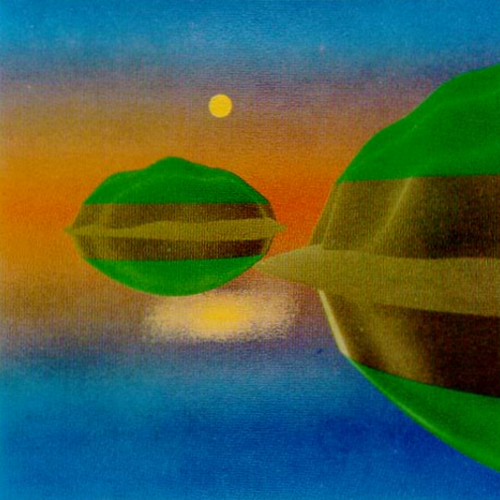
\includegraphics[scale=0.185]{figures/Vectorized_Procedural_Models_for_Natural_Terrain_-_Max_1981-006_1.png}
	\label{fig:max1981:1}
 }
 \hfill
 \subtop[]
 {
  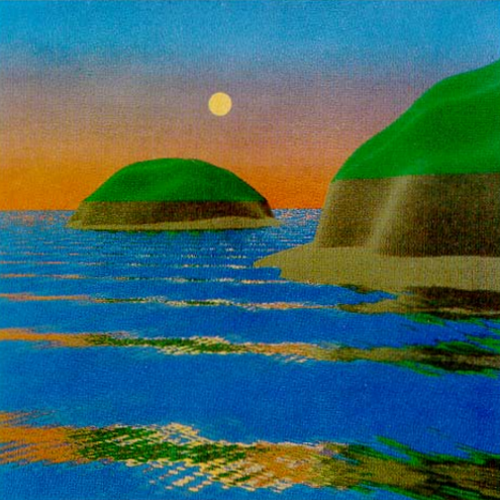
\includegraphics[scale=0.185]{figures/Vectorized_Procedural_Models_for_Natural_Terrain_-_Max_1981-007_1.png}
	\label{fig:max1981:2}
 }
 \hfill
 \subtop[]
 {
  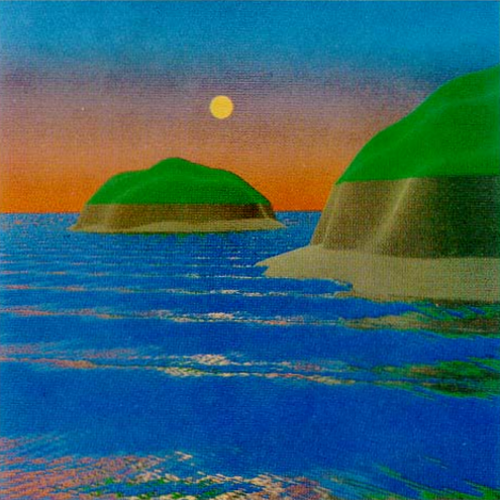
\includegraphics[scale=0.185]{figures/Vectorized_Procedural_Models_for_Natural_Terrain_-_Max_1981-006_2.png}
	\label{fig:max1981:3}
 }
 \hfill
 \subtop[]
 {
  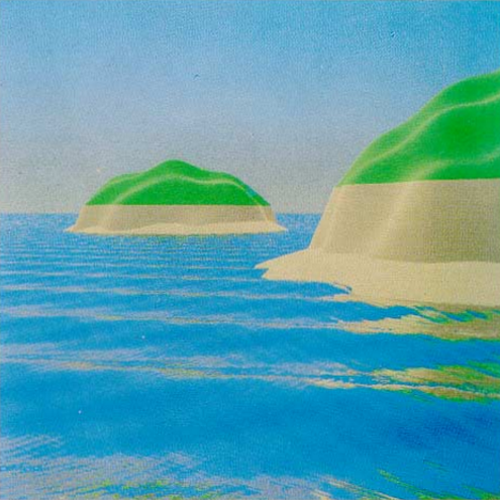
\includegraphics[scale=0.185]{figures/Vectorized_Procedural_Models_for_Natural_Terrain_-_Max_1981-007_2.png}
	\label{fig:max1981:4}
 }
\caption{\subcaptionref{fig:max1981:1}~Still water near sunset.
\subcaptionref{fig:max1981:2} One reflection from waves.
\subcaptionref{fig:max1981:3} Two reflections from waves.
\subcaptionref{fig:max1981:4} Early afternoon, two reflections from waves.
Source:~\citet{Max:1981}}
\label{fig:max1981}
\end{figure}
%
% \begin{figure}
% \begin{tabular}{cc}
% \subtop[sf1]{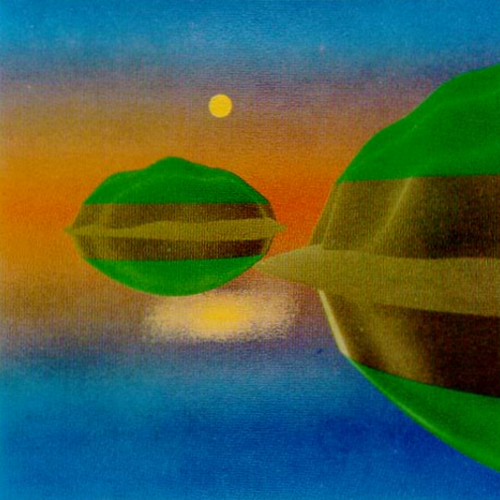
\includegraphics[scale=0.25]{figures/Vectorized_Procedural_Models_for_Natural_Terrain_-_Max_1981-006_1.png}} & \subtop[sf2]{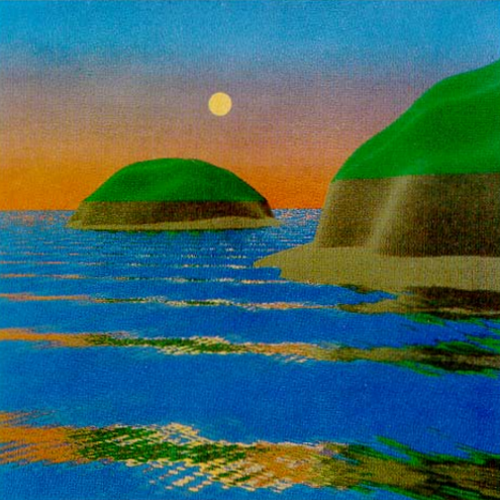
\includegraphics[scale=0.25]{figures/Vectorized_Procedural_Models_for_Natural_Terrain_-_Max_1981-007_1.png}}\\
% \subtop[sf3]{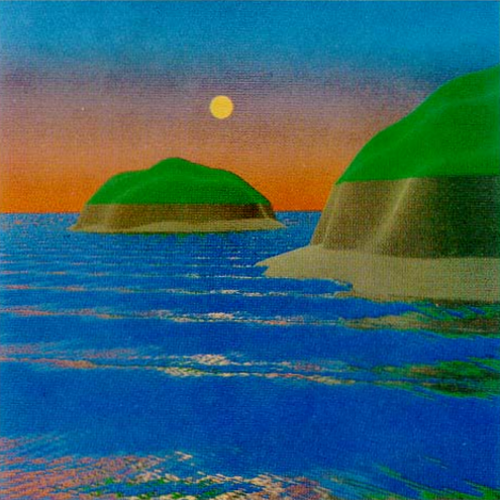
\includegraphics[scale=0.25]{figures/Vectorized_Procedural_Models_for_Natural_Terrain_-_Max_1981-006_2.png}} & \subtop[sf4]{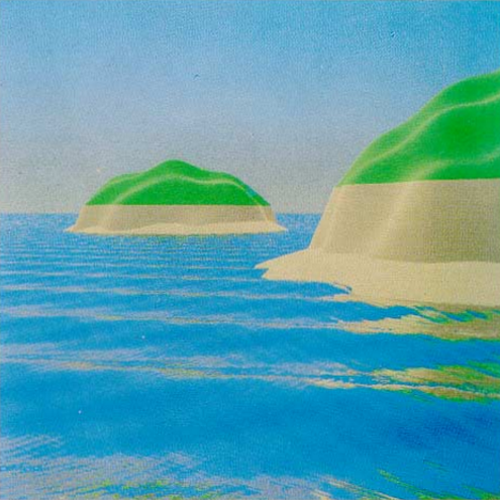
\includegraphics[scale=0.25]{figures/Vectorized_Procedural_Models_for_Natural_Terrain_-_Max_1981-007_2.png}}
% \end{tabular}\hfill
% % \begin{tabular}{c}
% % \subtop[sf4]{\rule{0.2\linewidth}{50pt}}\\
% % \subtop[sf5]{\rule{0.2\linewidth}{50pt}}
% % \end{tabular}\hfill
% \begin{tabular}[m]{c}
% \subtop[sf5]{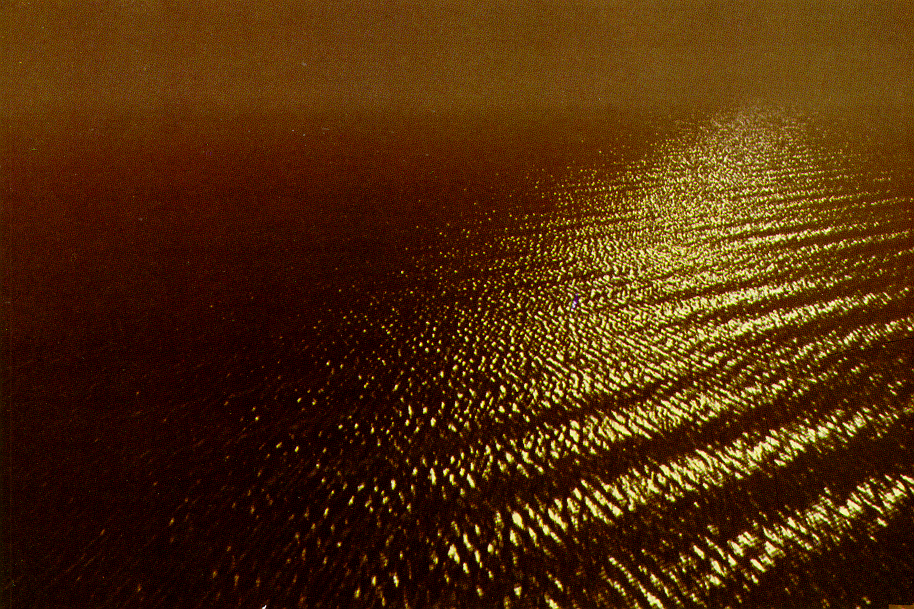
\includegraphics[scale=0.25]{figures/An_Image_Synthesizer_-_Perlin_1985-021.png}}
% \end{tabular}
% \caption{BRAK}
% \end{figure}
%
Parametric models are generally bound to the spatial domain, where they
generate and animate the ocean surface by means of a sum of periodical functions
which evolve throughout time using a phase difference. One of the earliest works
in this realm of computer graphics has been done by~\citet{Max:1981}. The ocean
surface is represented as a height map, where for each point $(x,z)$ at time $t$
the height is computed as a sum of sinusoids:
\begin{equation}
h(x,z,t) = y + \sum_{i=1}^N A_i \cos (l_i x + m_i z - \omega_i t)
\end{equation}
where $y$ is the mean height of the free surface, $N$ is the number of waves,
$A_i$ is the amplitude of the $i$th wave, $\omega_i$ its angular frequency,
and $\mvec{k}_i = (l_i, m_i)$ its \wavevector which defines the
travelling direction of the wave. For the sum of waves to achieve a
realistic shape, \citeauthor{Max:1981} applies linear wave theory \citep{book:airy1845tides}:
the waves on the water surface are assumed to be dominated by gravity, the wave
amplitudes are assumed to be small in relation to the size of the water body,
and the water body is assumed to have infinite depth. Then, according to linear
wave theory, it follows that the \wavenumber $k=\norm{\mvec{k}}$ and the angular
frequency $\omega$ are related by $\omega^2=kg$, where $g=9.81$ denotes earth's
gravity. Results obtained by~\citeauthor{Max:1981} are shown in
Figure~\ref{fig:max1981}.
%
% \begin{figure}[b]
%  \centering
%  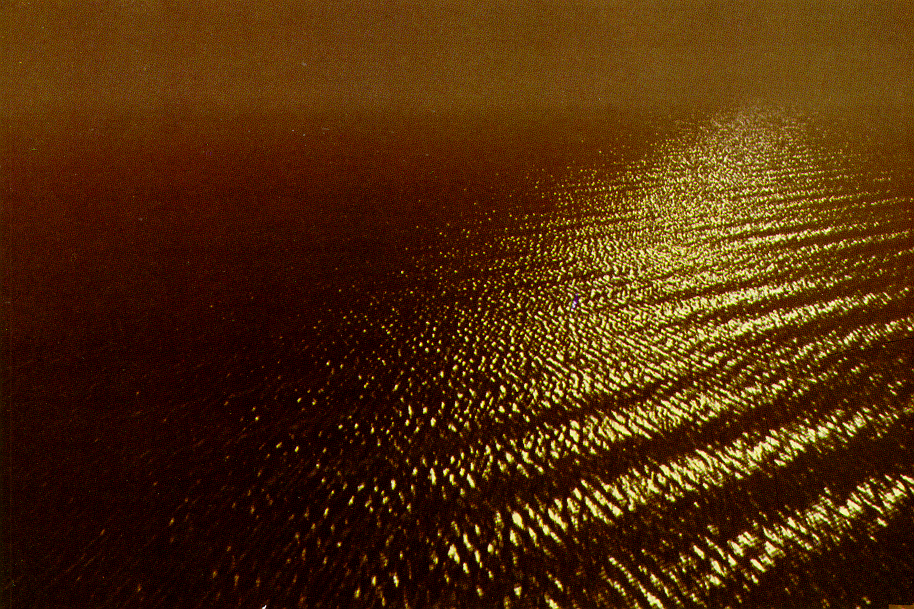
\includegraphics[scale=0.15]{figures/An_Image_Synthesizer_-_Perlin_1985-021.png}
%  \caption{Ocean sunset. Source:~\cite{Perlin:1985}}
% \label{fig:perlin1985}
% \end{figure}
%
Both~\citet{Schachter:1980} and~\citet{Perlin:1985} developed similar approaches,
but instead of generating any actual geometry they simply distort the normal
vectors of given surfaces.
% Results obtained by~\citeauthor{Perlin:1985} are shown in Figure~\ref{fig:perlin1985}.
%
\begin{figure}[t]
 \centering
 \subtop[]
 {
  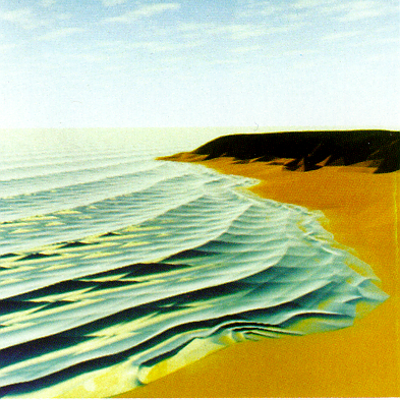
\includegraphics[scale=0.25]{figures/Modeling_Waves_and_Surf_-_Peachey_1986-009.png}
	\label{fig:peachey1986:1}
 }
 \hfill
 \subtop[]
 {
  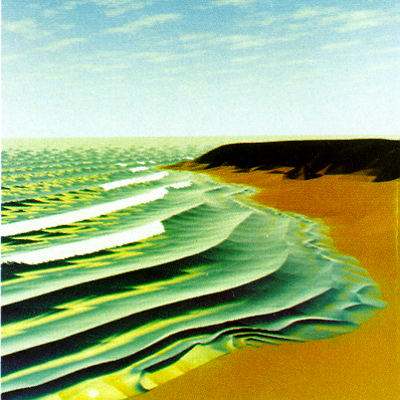
\includegraphics[scale=0.25]{figures/Modeling_Waves_and_Surf_-_Peachey_1986-010.png}
	\label{fig:peachey1986:2}
 }
 \hfill
 \subtop[]
 {
  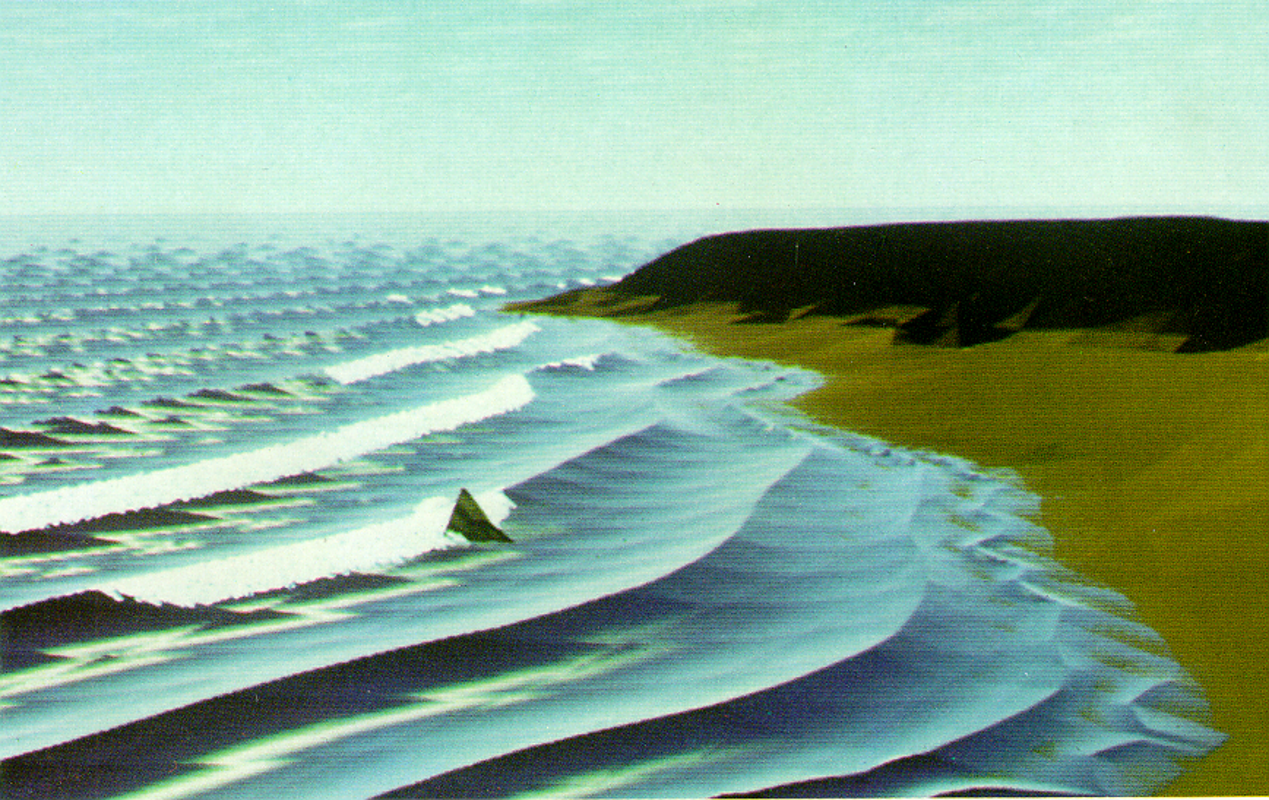
\includegraphics[scale=0.125]{figures/Modeling_Waves_and_Surf_-_Peachey_1986-012.png}
	\label{fig:peachey1986:3}
 }
 \caption{\subcaptionref{fig:peachey1986:1}~Waves on the beach.
\subcaptionref{fig:peachey1986:2}~Breaking waves on the beach.
\subcaptionref{fig:peachey1986:3}~Breaking waves with obstacle.
Source:~\citet{Peachey:1986}}
\label{fig:peachey1986}
\end{figure}
%

The assumption of infinite depth restricts the above methods to deep water,
they are unable to mimic the behaviour of waves as they approach the shore.
The transition of waves into shallow water is the cause for phenomena such
as the steepening and eventual breaking of waves, as well as for wave
refraction \citep{book:mei1989}. The latter describes the tendency of wavefronts
to align themselves
parallel to the sloping beach regardless of their initial orientation.
The underlying cause is the dependency of wave propagation speed on water depth,
where waves move more slowly in shallow water. The part of a wave front which
enters shallow water first is decelerated, the remainder of the wave still
in deeper water will move faster, as a result the wave front will be turned
parallel to the line of transition into shallow water.

\citet{Peachey:1986}, still in the realm of linear
wave theory, simulates waves near the shore through the relationship
$\omega^2=kg\tanh (kh)$, where $h$ is the water depth. Waves in shallow
water increase their steepness with declining water depth, \citeauthor{Peachey:1986}
therefore interpolates between a gentle sinusoidal wave form with long throughs
and rounded crests, and short choppy waves with sharp crests. To recreate the
appearance of waves near the breaking point, \citeauthor{Peachey:1986} steepens the front
of the crests of such waves even more, and stretches out the back of the crests,
giving the wave profile an asymmetric form.
Additionally, particle systems are added to generate spray wherever waves break or
collide with partially submerged obstacles.
Results of \citet{Peachey:1986} are shown in Figure~\ref{fig:peachey1986}.
%
\begin{figure}[p]
\begin{tikzpicture}
\begin{axis}[
	width=\textwidth,
	height=0.45\textwidth,
	domain=0:40,
	%xmin = 0,
	%xmax = 40,
	%axis equal,
	xtick=\empty,
	%ytick=\empty,
	%y tick label style={anchor=west,xshift=\pgfkeysvalueof{/pgfplots/major tick length}},
	yticklabels={$kA=0.2$,$kA=0.7$,$kA=1.0$,$kA=1.3$},
	ytick={12,8,4,0} 
	]
\addplot[samples=300,domain=0:40] ({x+0.2*sin(deg(1*x-sqrt(9.81*1)*0))}, {12-0.2*cos(deg(1*x-sqrt(9.81*1)*0))});
\addplot[samples=300,domain=0:40] ({x+0.7*sin(deg(1*x-sqrt(9.81*1)*0))}, { 8-0.7*cos(deg(1*x-sqrt(9.81*1)*0))});
\addplot[samples=300,domain=0:40] ({x+1.0*sin(deg(1*x-sqrt(9.81*1)*0))}, { 4-1.0*cos(deg(1*x-sqrt(9.81*1)*0))});
\addplot[samples=300,domain=0:40] ({x+1.3*sin(deg(1*x-sqrt(9.81*1)*0))}, { 0-1.3*cos(deg(1*x-sqrt(9.81*1)*0))});
\end{axis}
\end{tikzpicture}
\caption{Example waves with different $kA$. One can see that the wave crest gets more pronounced as $kA$ grows,
with the wave intersecting itself when $kA > 1$.}
\label{fig:trochoid:crests}
\end{figure}
%
%
\begin{figure}[p]
 \centering
 \subtop[]
 {
  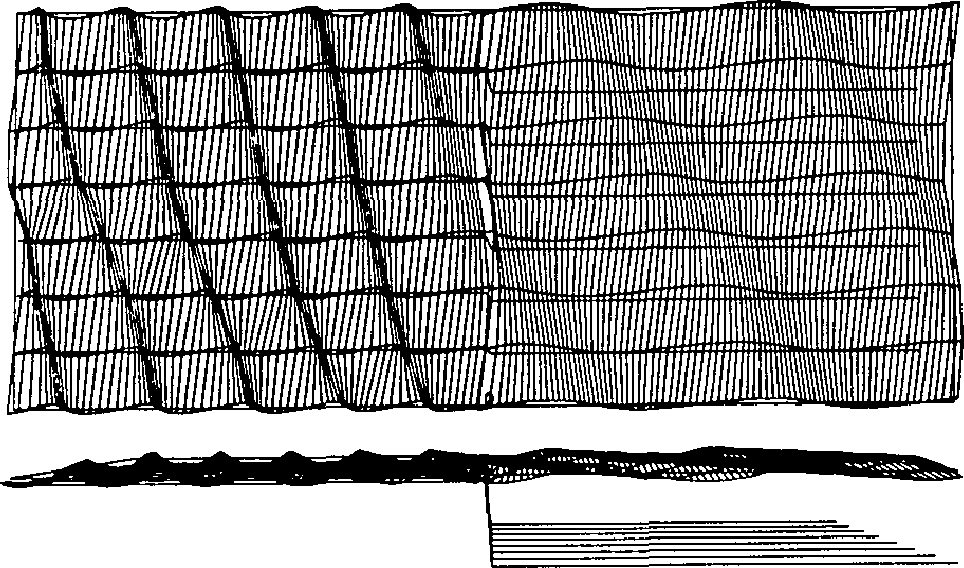
\includegraphics[scale=0.175]{figures/A_Simple_Model_of_Ocean_Waves_-_Fournier_1986-004_1.png}
	\label{fig:fournier1986:refraction:1}
 }
 \hfill
 \subtop[]
 {
  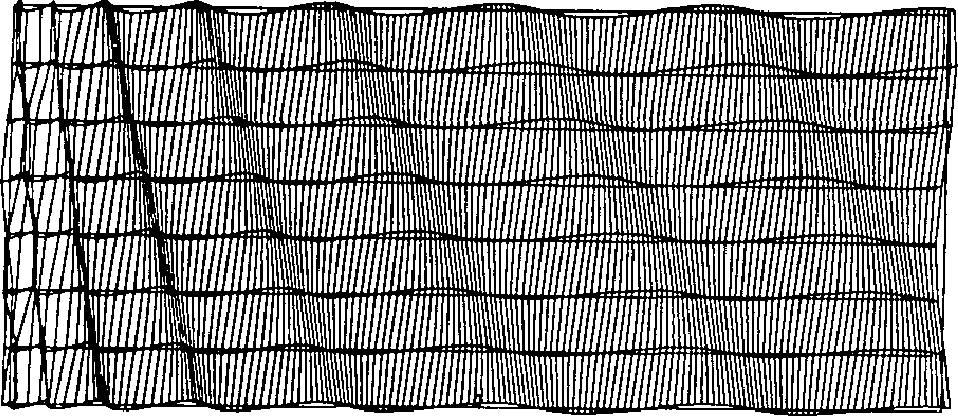
\includegraphics[scale=0.175]{figures/A_Simple_Model_of_Ocean_Waves_-_Fournier_1986-004_2.png}
	\label{fig:fournier1986:refraction:2}
 }
 \hfill
 \subtop[]
 {
  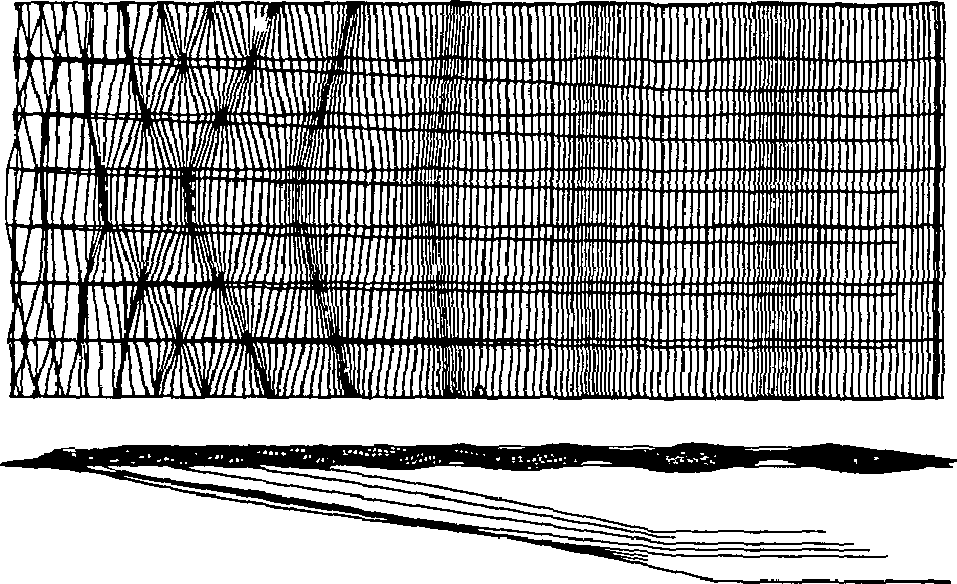
\includegraphics[scale=0.175]{figures/A_Simple_Model_of_Ocean_Waves_-_Fournier_1986-005_1.png}
	\label{fig:fournier1986:refraction:3}
 }
 \caption{The refraction of waves.
\subcaptionref{fig:fournier1986:refraction:1} Two bottoms of constant depth, the
\wavelengths are halved as the waves reach the shallow bottom on the left.
\subcaptionref{fig:fournier1986:refraction:2} The beach slopes gently down from
the left. One can see the wave fronts aligning themselves with the beach.
\subcaptionref{fig:fournier1986:refraction:3} An undersea valley that affects
both, the \wavelengths as well as the travelling direction of the waves.
Source:~\citet{Fournier:1986}}
\label{fig:fournier1986:refraction}
\end{figure}
%
%
\begin{figure}[p]
 \centering
 \subtop[]
 {
  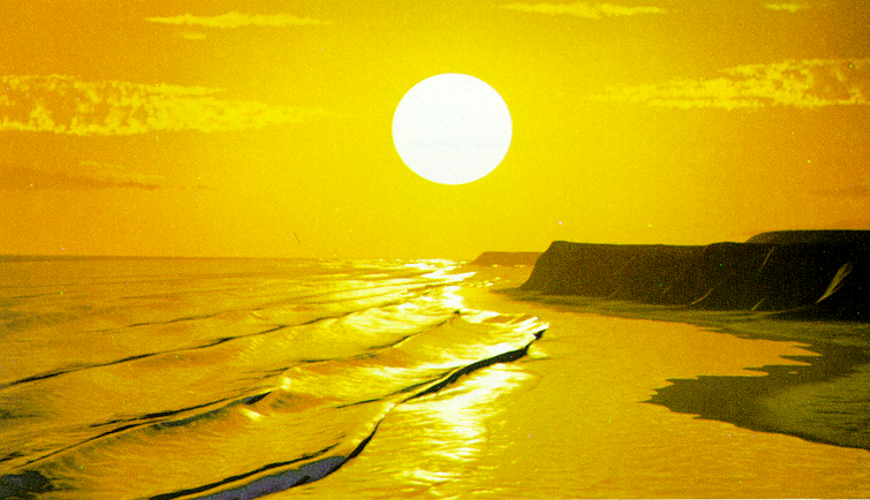
\includegraphics[scale=0.225]{figures/A_Simple_Model_of_Ocean_Waves_-_Fournier_1986-008.png}
	\label{fig:fournier1986:results:1}
 }
 \hfill
%  \subtop[]
%  {
%   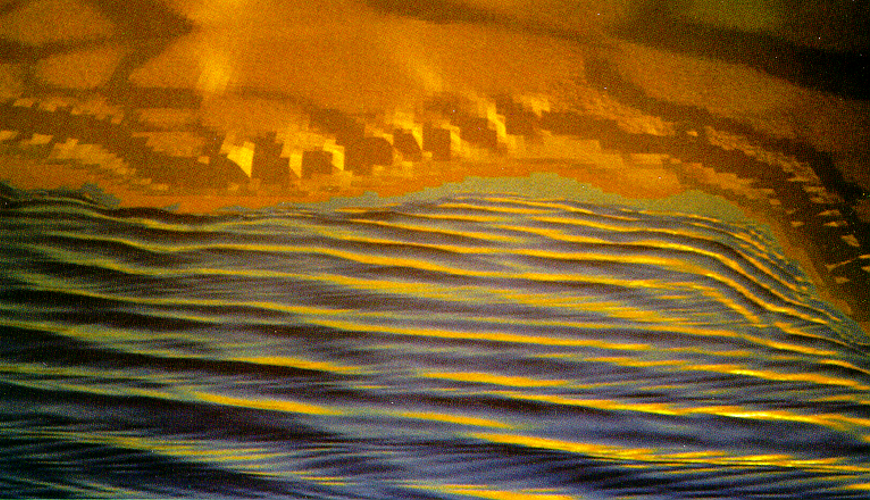
\includegraphics[scale=0.225]{figures/A_Simple_Model_of_Ocean_Waves_-_Fournier_1986-010.png}
% 	\label{fig:fournier1986:results:2}
%  }
%  \subtop[]
%  {
%   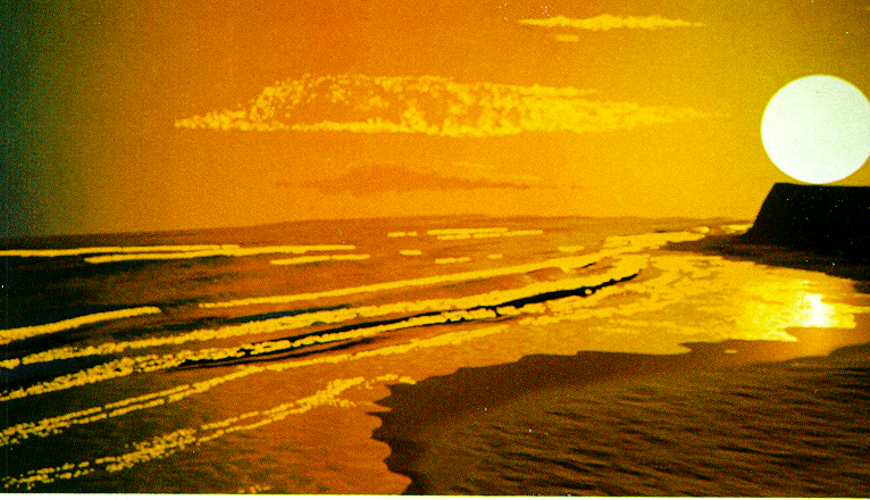
\includegraphics[scale=0.225]{figures/A_Simple_Model_of_Ocean_Waves_-_Fournier_1986-011.png}
% 	\label{fig:fournier1986:results:3}
%  }
%  \hfill
 \subtop[]
 {
  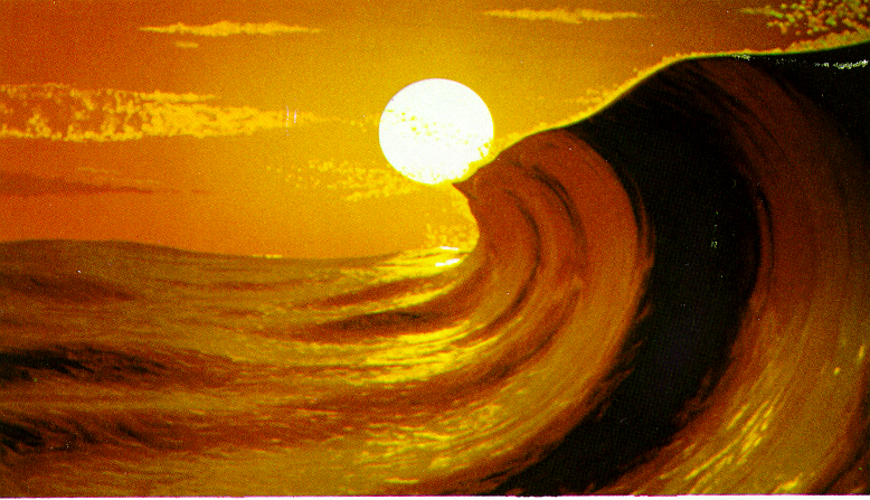
\includegraphics[scale=0.225]{figures/A_Simple_Model_of_Ocean_Waves_-_Fournier_1986-013.png}
	\label{fig:fournier1986:results:4}
 }
 \caption{
 \subcaptionref{fig:fournier1986:results:1} Breaking waves on the shore, where the crests take the shape of the shore.
%  \subcaptionref{fig:fournier1986:results:2} Wave refraction.
%  \subcaptionref{fig:fournier1986:results:3} Waves with spray and foam.
 \subcaptionref{fig:fournier1986:results:4} A large breaking wave.
 Source:~\citet{Fournier:1986}
 }
 \label{fig:fournier1986:results}
\end{figure}
%
%

Instead of using sinusoids,~\citet{Fournier:1986} build on Gerstner's work
\citep{Gerstner:1809, Rankine:1863} to synthesize waves. Gerstner waves assume
a water surface dominated by gravity and an incompressible water body of
infinite depth. A single wave may be written as follows:
\begin{align}
\mvec{x} &= \mvec{x}_0 - \frac{\mvec{k}}{\norm{\mvec{k}}} A \sin\left(\mvec{k}\cdot\mvec{x}_0-\omega t\right)\\
y &= y_0 - A \cos\left(\mvec{k}\cdot\mvec{x}_0-\omega t\right)
\end{align}
where $\mvec{x}=(x,z)$ denotes the horizontal coordinate and $y$ the
vertical coordinate of the wave particle at time $t$, with $\mvec{x}_0$ and $y_0$ its horizontal
and vertical position at rest respectively. As before, $A$ is the amplitude,
$\mvec{k}$ the \wavevector and $\omega$ the wave's angular frequency. Given the
\wavenumber $k=\norm{\mvec{k}}$, the term $kA$ defines the sharpness of the wave
crest. With $kA<1$ the wave takes the form of an upside-down trochoid, with
$kA=1$ the form of an upside-down cycloid, and with $kA>1$ the wave intersects
itself, an undesireable effect which does not resemble real waves.
See Figure~\ref{fig:trochoid:crests} for waves with different $kA$.
We may write the sum of Gerstner waves involving $N$ components as follows:
\begin{align}
\mvec{x} &= \mvec{x}_0 - \sum_i^N\frac{\mvec{k}_i}{\norm{\mvec{k_i}}} A_i \sin\left(\mvec{k}_i\cdot\mvec{x}_0-\omega_i t\right)\\
y &= y_0 - \sum_i^N A_i \cos\left(\mvec{k}_i\cdot\mvec{x}_0-\omega_i t\right)
\end{align}
%

To model waves in shallow water, \citet{Fournier:1986} extend the Gerstner
wave model in two ways. First, waveparticle motion takes the underlying sea
bed into account, allowing for waves to be refracted i.e. to change their \wavelength,
their speed and their direction of travel based on water depth, see Figure~\ref{fig:fournier1986:refraction}.
Second, the circular orbit of Gerstner waves approaching the shore is
transformed into an elliptical orbit, which allows to approximate the form of
steepening and eventually breaking waves.
Results of \citeauthor{Fournier:1986} are shown in Figure~\ref{fig:fournier1986:results}.
%
\begin{figure}
 \centering
 \subtop[]
 {
  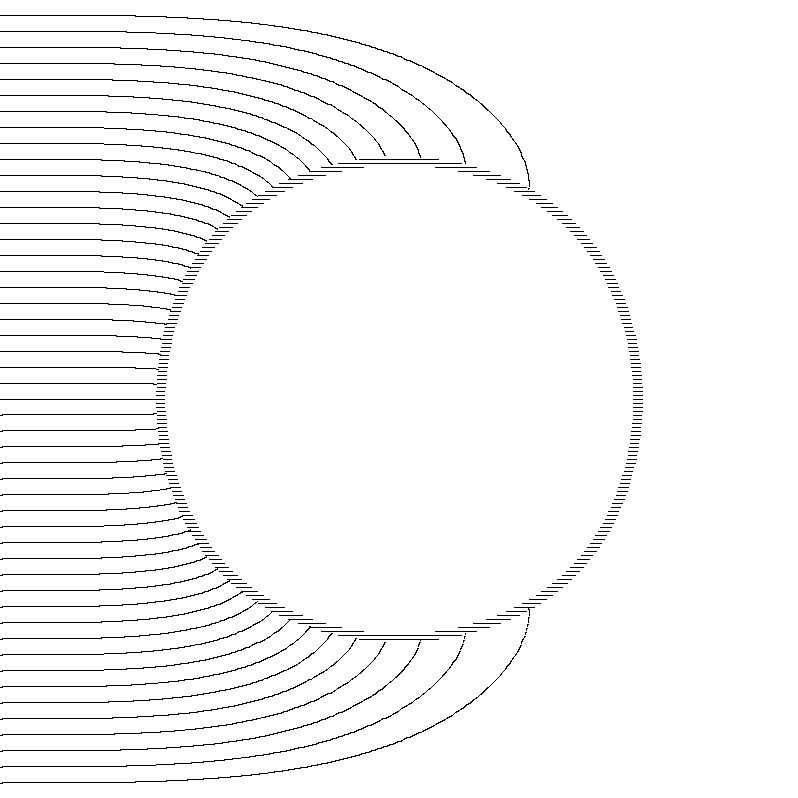
\includegraphics[width=0.2\textwidth]{figures/A_phenomenological_model_of_coastal_scenes_based_on_physical_considerations_-_Gonzato_1997-051.png}
	\label{fig:gonzato1997:results:1}
 }
 \hfill
 \subtop[]
 {
  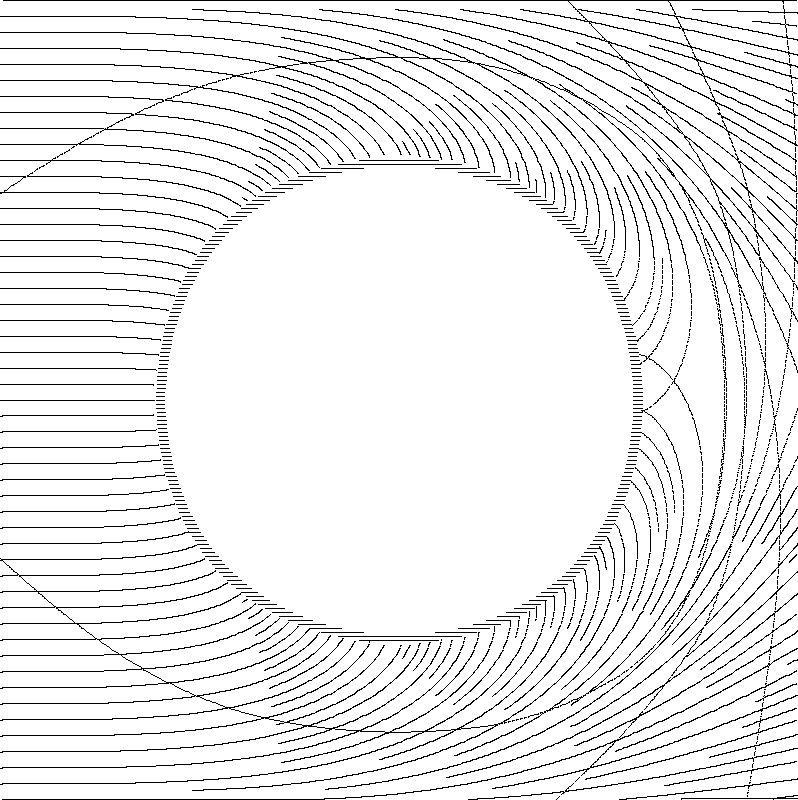
\includegraphics[width=0.2\textwidth]{figures/A_phenomenological_model_of_coastal_scenes_based_on_physical_considerations_-_Gonzato_1997-055.png}
	\label{fig:gonzato1997:results:2}
 }
 \hfill
 \subtop[]
 {
  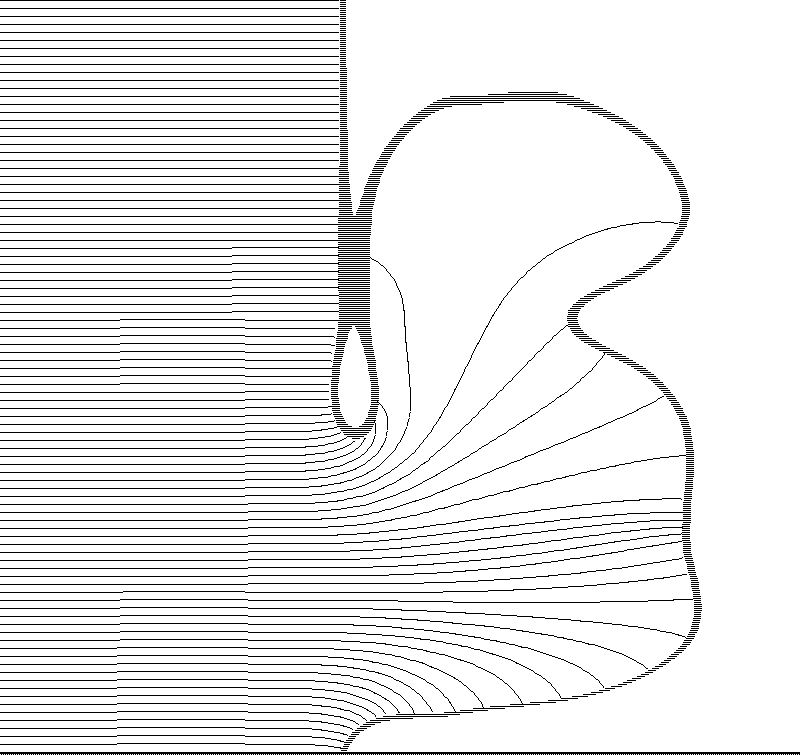
\includegraphics[width=0.2\textwidth]{figures/A_phenomenological_model_of_coastal_scenes_based_on_physical_considerations_-_Gonzato_1997-052.png}
	\label{fig:gonzato1997:results:3}
 }
 \hfill
 \subtop[]
 {
  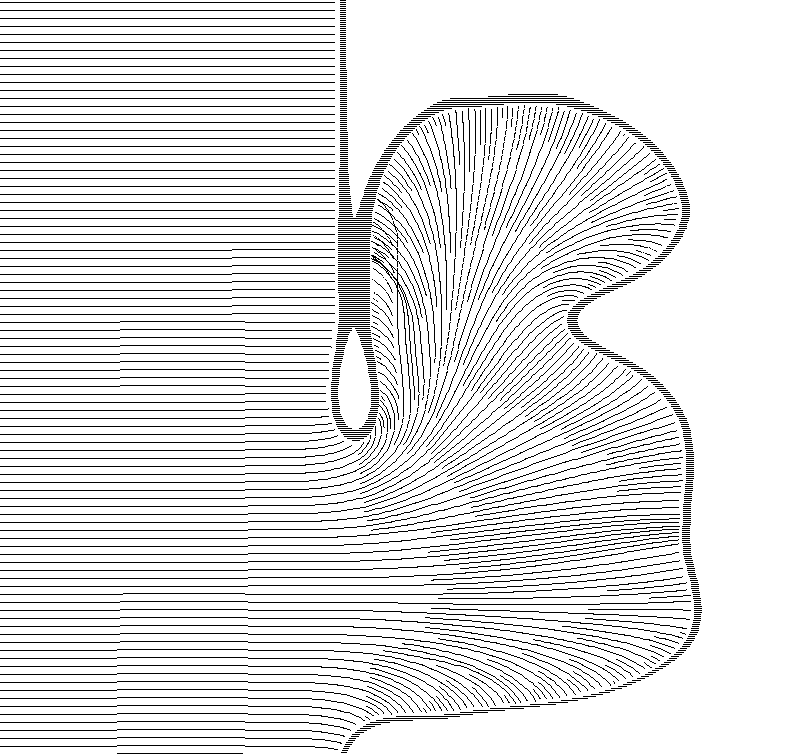
\includegraphics[width=0.2\textwidth]{figures/A_phenomenological_model_of_coastal_scenes_based_on_physical_considerations_-_Gonzato_1997-056.png}
	\label{fig:gonzato1997:results:4}
 }
 \caption{
 \subcaptionref{fig:gonzato1997:results:1} Wave Trace of an island.
 \subcaptionref{fig:gonzato1997:results:2} Dynamic Wave Trace of the same island.
 \subcaptionref{fig:gonzato1997:results:3} Wave Trace of a bay.
 \subcaptionref{fig:gonzato1997:results:4} Dynamic Wave Trace of the same bay.
 Source:~\citet{Gonzato:1997}
 }
 \label{fig:gonzato1997:results}
\end{figure}
%

\citet{Ts'o:1987} compute wave propagation near the shore with an algorithm
called \emph{wave tracing}, which launches orthogonal wave rays from the open
sea along the direction of wave propagation. Wave refraction is computed based
on Snell's law~\citep{book:huygenstreatiseonlight}, the wave trains are traced
inside a uniform grid.
In case rays tracing the waves path diverge
significantly from a straight line, there may remain undersampled areas,
leading to parts of the surface lacking detail. \citet{Gonzato:1997} improve
upon this by generating new rays in undersampled areas, allowing their
\emph{dynamic wave tracing} algorithm to more densely sample the water surface
surrounding islands and the water surface inside bays. See Figure
\ref{fig:gonzato1997:results} for a comparison between wave tracing and
dynamic wave tracing. Moreover,
\citeauthor{Gonzato:1997} modify the wave model to include plunging breaking
waves. Three additional functions achieve said goal.
First, a stretch function imitates Biesel's law~\citep{Biesel:1952} by
progressively stretching the wave on the crest along its major axis. Second and
third, an orientation and a displacement function rotate and translate
the wave's crest downwards, towards the water surface below the crest.
\citet{Gonzato:2000} augment their work with the inclusion of wave diffraction
caused by jetties, and with the addition of capillary waves which are modeled
using fractal noise.

Parametric models are well suited to model propagating water fronts, where a
small number of \wavenumbers may suffice to obtain satisfactory results.
Because one has basically to select the involved \wavelengths and amplitudes
by trial and error, it follows that parametric models are not particularly
eligible to represent an agitated water surface, as it would involve a
significant higher number of waves. The user may have a hard time assembling a
meaningful number of \wavenumbers and amplitudes, with the result being
potentially infeasible because of the accumulated computational cost.
%
%
\section{Spectral Models}
%
Oceanographic research employs~\emph{wave spectra} to model the deep ocean
\citep{book:kinsman2002wind}. The sea is assumed as a linear superposition of
sinusoids with many different \wavelengths, frequencies and phases, travelling
in different directions. The wave spectrum gives the distribution of wave energy
among different wave frequencies or \wavelengths.
Given horizontal coordinate $\mvec{x}$, according to
\citet{course:simulatingocean} we may compute the vertical coordinate
at time $t$ via an \InvDiscreteFourierTransform as follows:
\begin{equation}
h(\mvec{x},t) = \sum_{\mvec{k}}A(\mvec{k},t)\mathrm{e}^{\mathrm{i}\transpose{\mvec{k}}\mvec{x}}
\label{eq:spectral_models}
\end{equation}
where $\mvec{k}$ represents the \wavevectors of the most significant frequency
components, and $A(\mvec{k},t)$ the amplitudes obtained from the wave
spectrum.
At this point we refer to Chapter~\ref{ch:background} for a more thorough
discussion of the theoretical background of wave spectra.
% At this point we refer to Sections \ref{sec:linear_theory_ocean_waves}
% and \ref{sec:random_sea} for a more thorough discussion of the theoretical
% background of wave spectra, whereas Section \ref{sec:random_sea_discretisation}
% explains Equation~\ref{eq:spectral_models} in detail. 
For now it shall suffice to give an overview of key properties of wave spectra. 

First, all wave spectra are static \citep{book:kinsman2002wind}.
Static in the sense, that a wave spectrum represents a certain sea
state based on parameters such as wind speed and the distance from shore. To
change the sea state requires the synthesis of a new wave spectrum. Thus, for
example, if one would like to simulate a calm sea which gets agitated as a storm
approaches, then one needs to generate a wave spectrum for each specific wind
speed, and optionally interpolate between those spectra.

Second, wave spectra are compact models which require only a small
number of input parameters defining the desired sea state
\citep{book:windgeneratedoceanwaves, book:kinsman2002wind}.
Since wave spectra
are homogeneous models, all parameters are uniform for the entire ocean surface,
there is no room for local variations as parametric models would allow. Wave
spectra assume the ocean surface to be dominated by the interplay of wind and
gravity, hence wind speed is the parameter common to all models. Another well
established parameter is~\emph{fetch}, which is the distance over which the wind
blows before it reaches the ocean patch the wave spectrum simulates. Water
depth, if supported by the wave spectrum model, is uniform like all other
parameters hence the sea bed is assumed planar and parallel to the ocean surface
at rest. It follows that no wave transitions from one water depth to another,
therefore no wave refraction may take place \citep{book:mei1989}.

Third, the \InvDiscreteFourierTransform may leverage the
\FastFourierTransform algorithm~\citep{Cooley:1965}, which makes the computation of
Equation~\ref{eq:spectral_models} most efficient. Hence, given the same
computational cost, it is possible for spectral models to involve way more
\wavenumbers in the sum of waves than parametric models could. Moreover, thanks to
the \DiscreteFourierTransform we get a seamless tileable surface.
The downside of the \FourierTransform is that the range and uniform sampling
density of spatial coordinates $\mvec{x}$ directly defines the set of \wavevectors
$\mvec{k}$ contributing to the sum of waves. In contrast to the
parametric models we are neither able to cherry-pick certain \wavevectors,
nor to omit a range of \wavevectors, nor to to exert some form of local control
where we modify the set of \wavevectors based on location $\mvec{x}$.
Despite those drawbacks, \citet{Mitchell:2005} and \citet{Thon:2000} still
argue that from an algorithmic point of view one should choose a spectral
approach over a parametric one. Only by computing the sum of waves with the
highly efficient \FastFourierTransform algorithm, one is able to include the
vast amount of \wavenumbers necessary to synthesize a strongly agitated ocean
surface.
%
\begin{figure}
 \centering
 \subtop[]
 {
  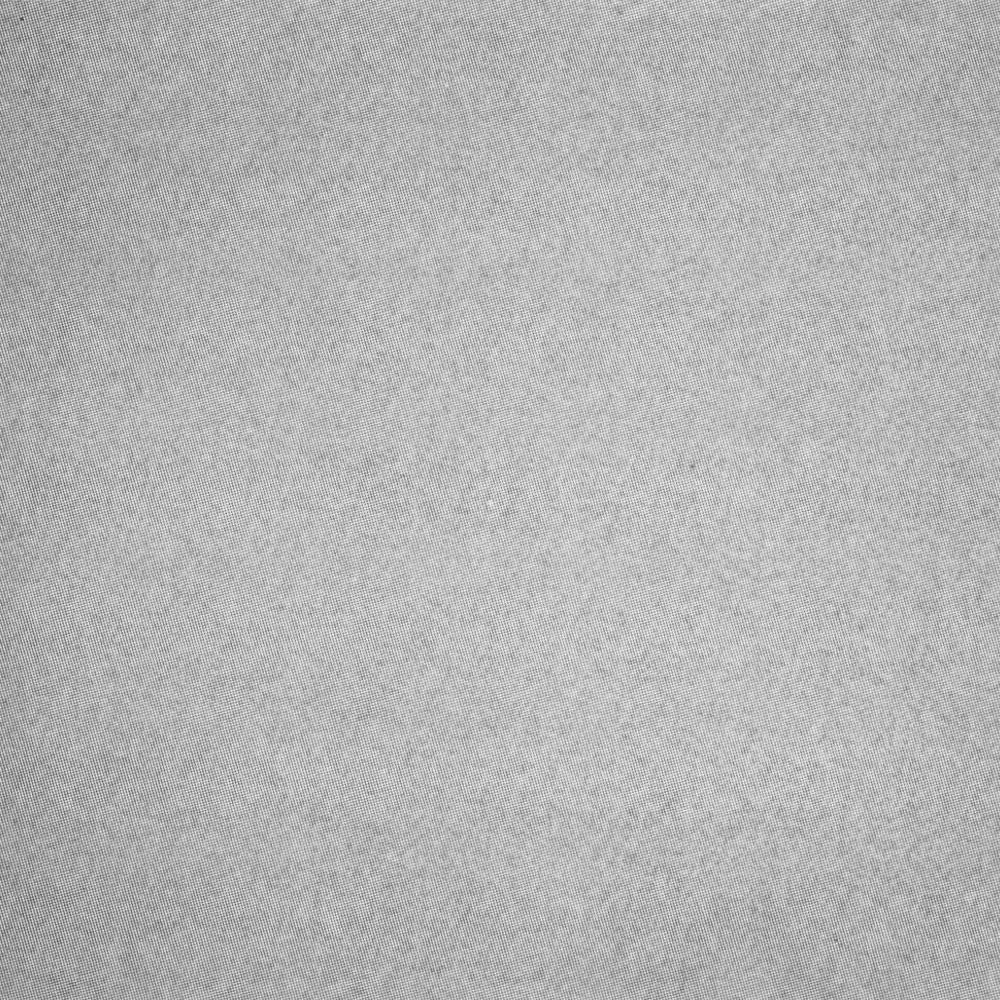
\includegraphics[scale=0.1125]{figures/Fourier_Synthesis_of_Ocean_Scenes_-_Mastin_1987-005_1.png}
	\label{fig:mastin_waves:1}
 }
 \hfill
 \subtop[]
 {
  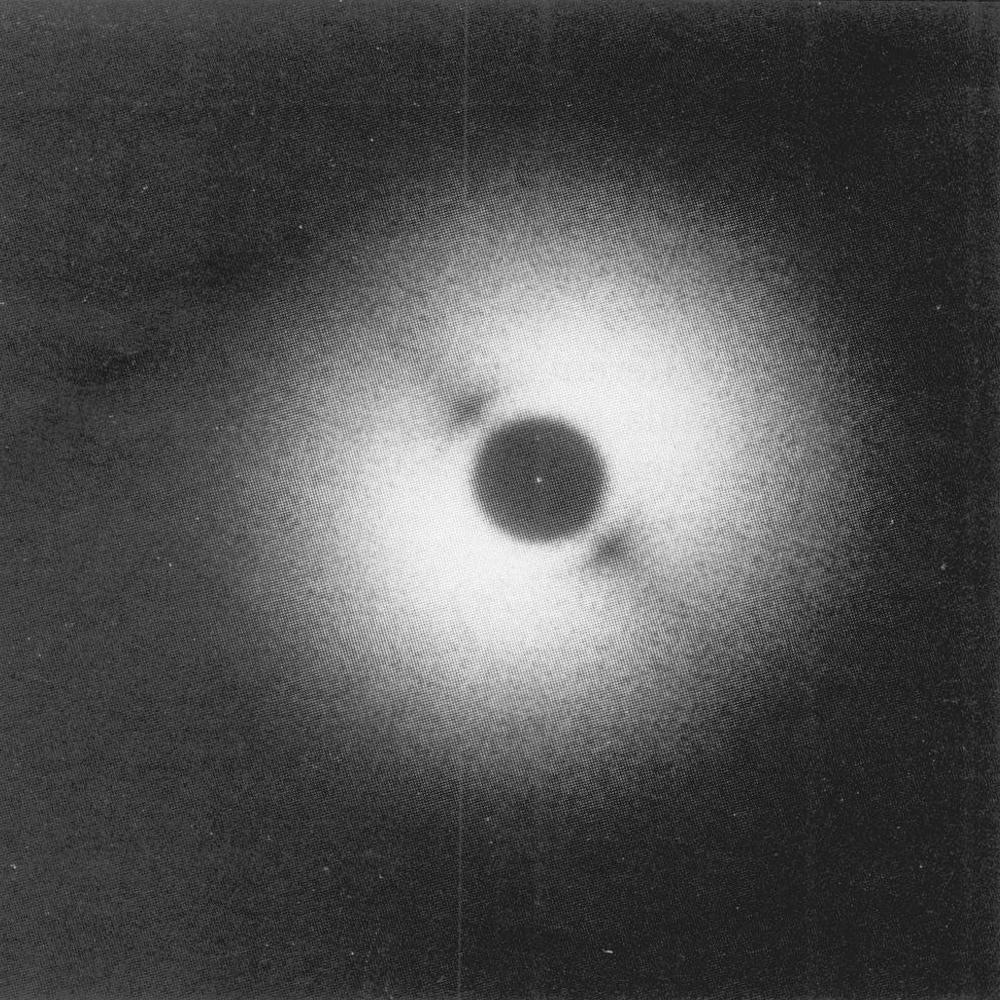
\includegraphics[scale=0.1125]{figures/Fourier_Synthesis_of_Ocean_Scenes_-_Mastin_1987-005_2.png}
	\label{fig:mastin_waves:2}
 }
 \hfill
 \subtop[]
 {
  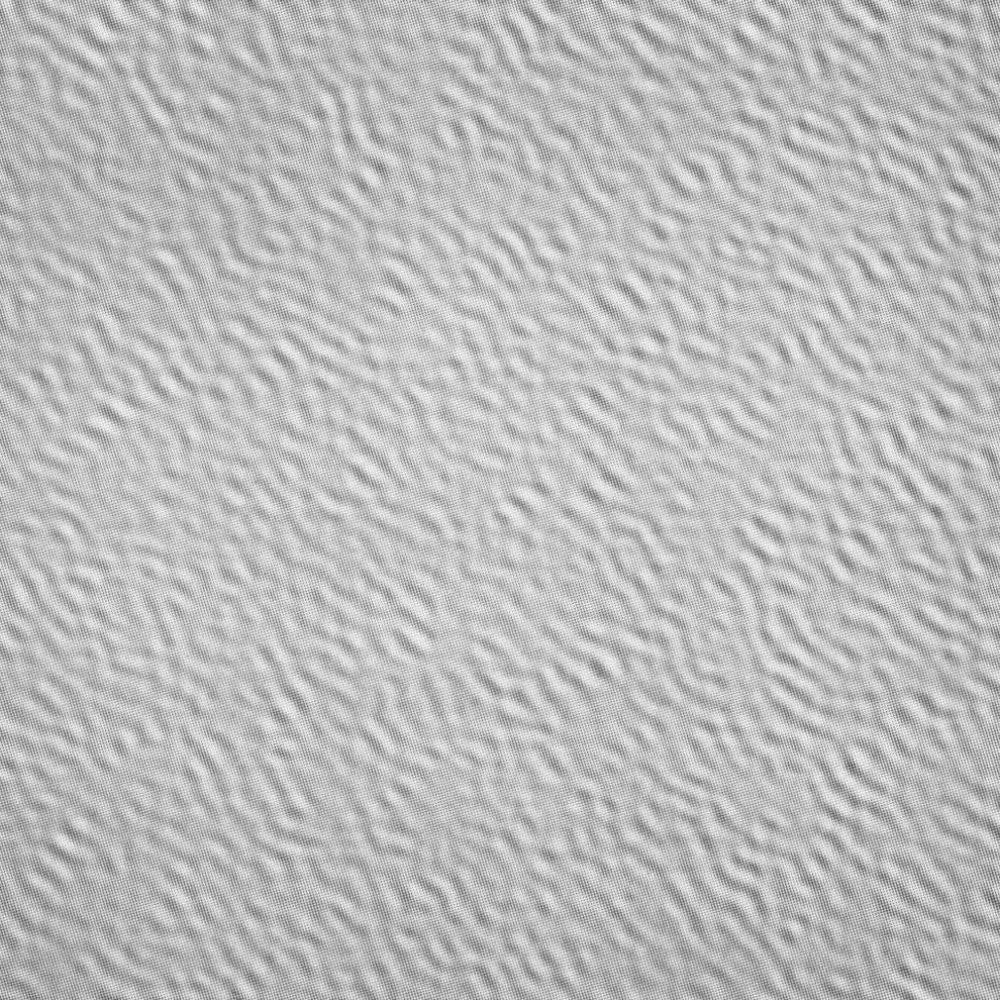
\includegraphics[scale=0.1125]{figures/Fourier_Synthesis_of_Ocean_Scenes_-_Mastin_1987-005_3.png}
	\label{fig:mastin_waves:3}
 }
 \hfill
 \subtop[]
 {
  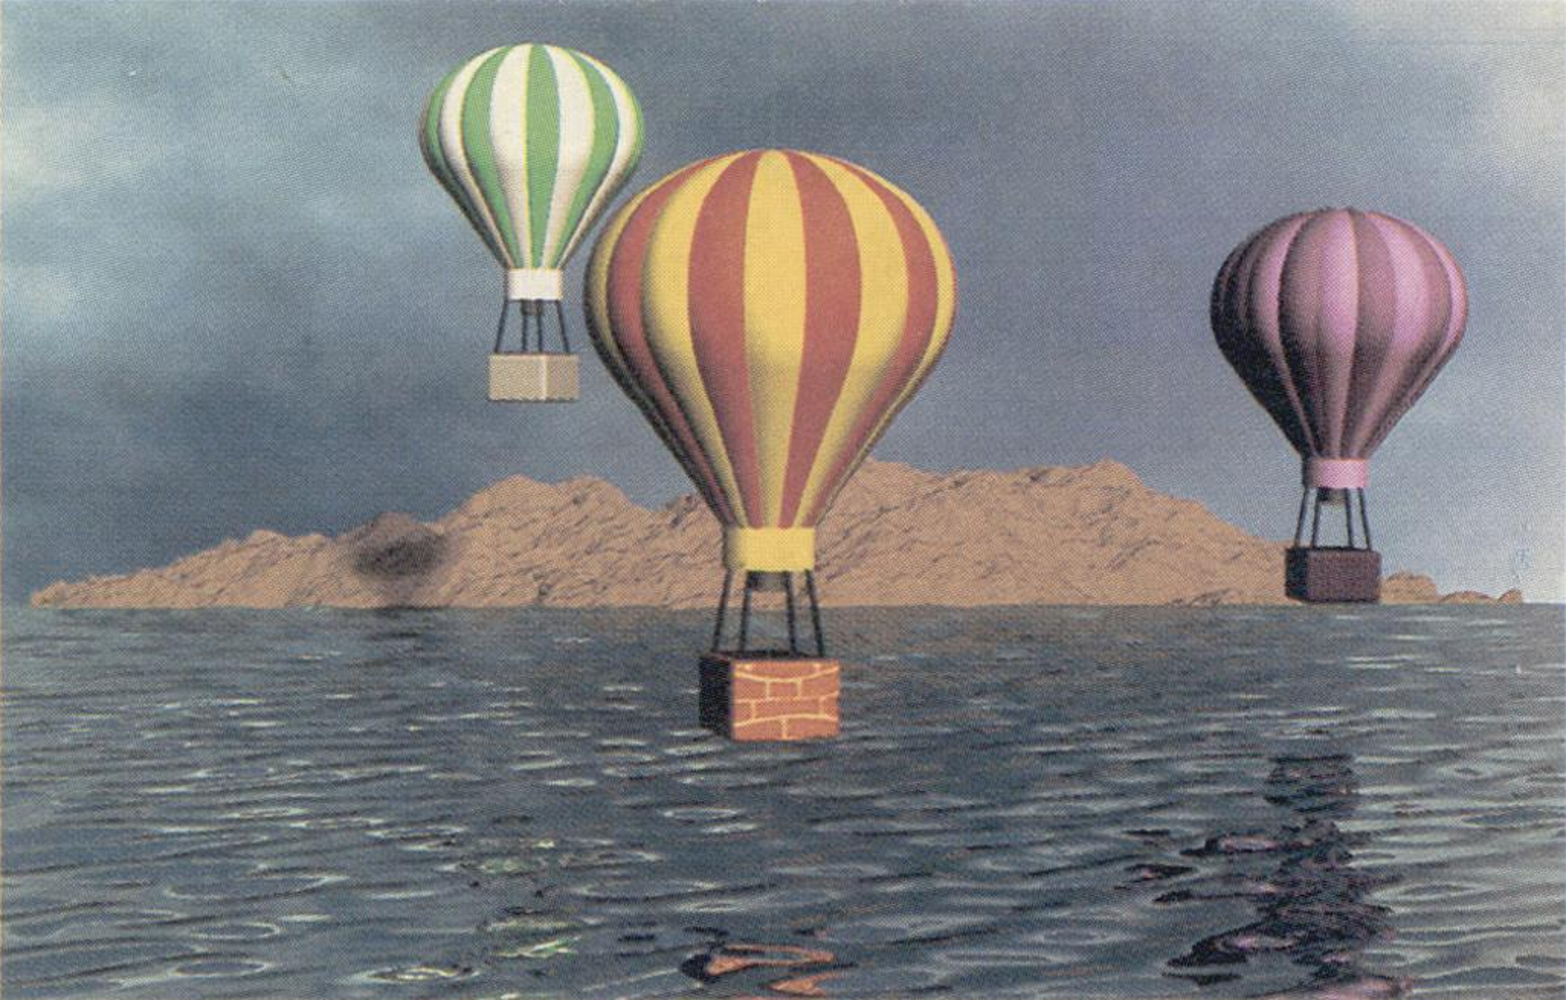
\includegraphics[scale=0.1125]{figures/Fourier_Synthesis_of_Ocean_Scenes_-_Mastin_1987-007_1.png}
	\label{fig:mastin_waves:4}
 }
 \caption{
\subcaptionref{fig:mastin_waves:1} White noise.
\subcaptionref{fig:mastin_waves:2} The Pierson-Moskowitz spectrum combined with the directional spreading function.
\subcaptionref{fig:mastin_waves:3} The synthesized heightfield.
\subcaptionref{fig:mastin_waves:4} Rendering of the sea surface.
Source: \citet{Mastin:1987}
}
\label{fig:mastin_waves}
\end{figure}
%

\citet{Mastin:1987} introduced wave spectra to computer graphics. Their approach
is a simple one: generate white noise to represent random amplitudes and phases,
then filter it with the Pierson-Moskowitz spectrum
\citep{article:PiersonMoskowitz1964} in frequency space. The Pierson-Moskowitz
spectrum gives wave energy per \wavenumber, but not its distribution across
\wavevectors. In short, there is no information telling in which direction the
waves are moving. Thus, \citeauthor{Mastin:1987} combine the Pierson-Moskowitz
spectrum with a \emph{directional spreading function}, namely the one proposed
in \citet{article:Hasselmann1980}. A directional
spreading function distributes wave energy across \wavevectors, where
the energy peak is usually to be found aligned with the wind direction and the
remaining energy fanning out at its sides. Results of \citet{Mastin:1987} are
shown in Figure~\ref{fig:mastin_waves}.
\citet{Premoze:2000} on the other hand make use of the JONSWAP spectrum
\citep{article:Hasselman1973}, as it allows for more varied ocean surfaces than
the Pierson-Moskowitz spectrum.
% An in-depth discussion of the Pierson-Moskowitz spectrum, the JONSWAP spectrum,
% as well as directional spreading functions is to be found in Section
% \ref{sec:1d_frequency_spectra}.
%
\begin{figure}
 \centering
 \subtop[]
 {
  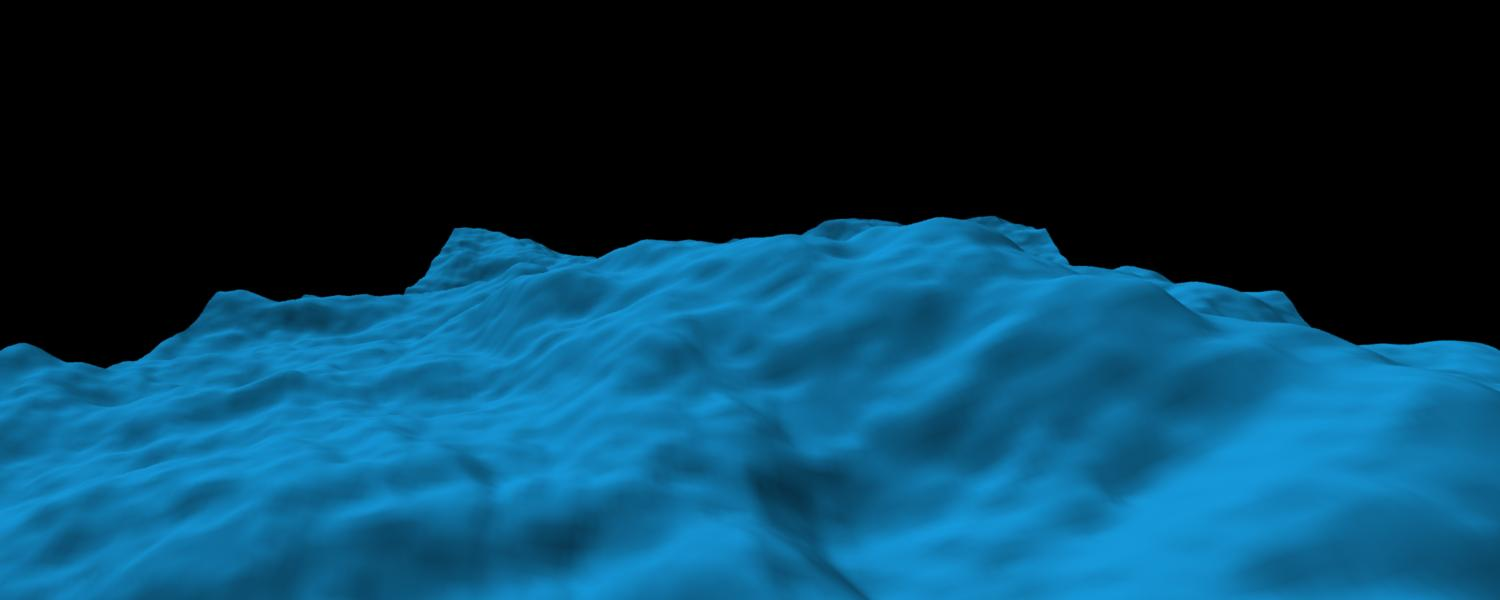
\includegraphics[scale=0.125]{figures/Simulating_Ocean_Water-012.png}
	\label{fig:tessendorf_choppy_waves:1}
 }
 \hfill
 \subtop[]
 {
  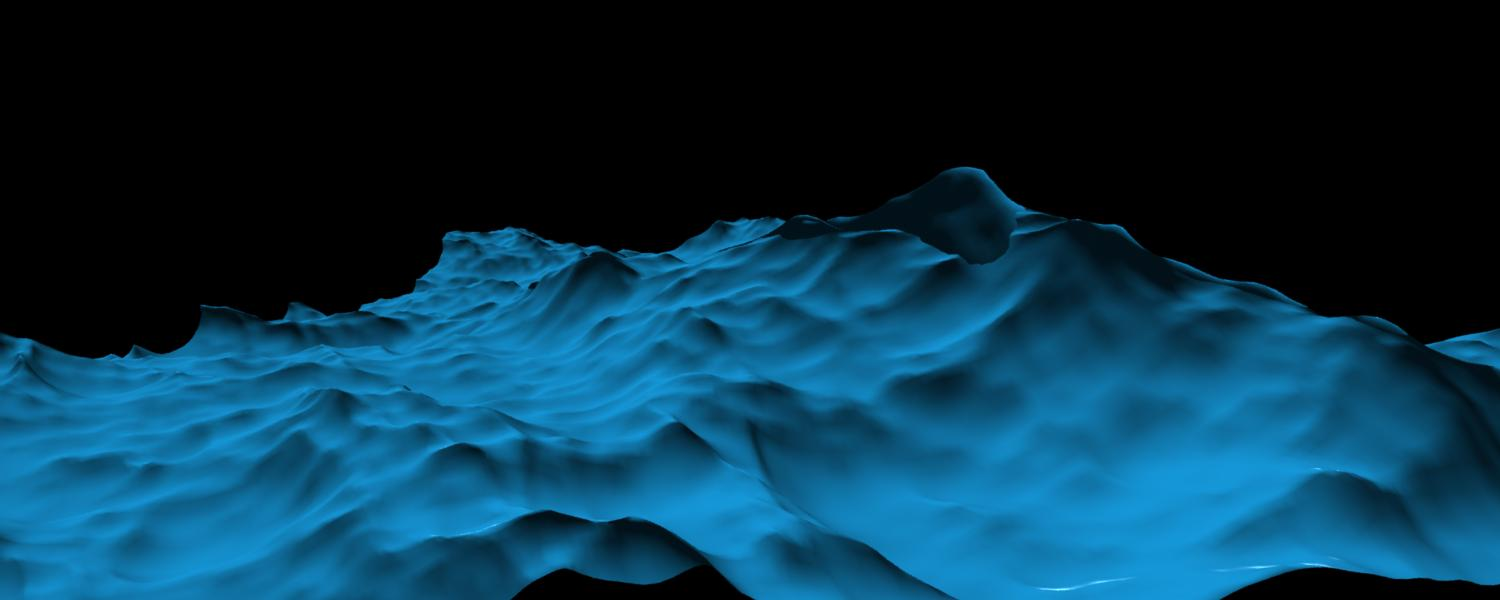
\includegraphics[scale=0.125]{figures/Simulating_Ocean_Water-013.png}
	\label{fig:tessendorf_choppy_waves:2}
 }
 \caption{
\subcaptionref{fig:tessendorf_choppy_waves:1} Ocean surface sythesized with the Phillips spectrum.
\subcaptionref{fig:tessendorf_choppy_waves:2} The same surface with the choppy wave algorithm applied.
Source: \citet{course:simulatingocean}
}
\label{fig:tessendorf_choppy_waves}
\end{figure}
%

One of the most known works in computer graphics related to wave spectra is
\citet{course:simulatingocean}. Therein, \citeauthor{course:simulatingocean}
describes how the ocean was brought to life for productions such as
\emph{Waterworld} and \emph{Titanic}. In contrast to \citeauthor{Mastin:1987},
\citeauthor{course:simulatingocean} does not use white noise, but Gaussian
random numbers, because waves in deep sea areas are often observed to follow a
Gaussian distribution. Moreover, \citeauthor{course:simulatingocean}
makes use of the Phillips spectrum, a spectrum devised by himself specifically
for computer graphics purposes, but loosely based on oceanographic research
published in \citet{article:Phillips1958,article:Phillips1985}.

Ocean surfaces based on wave spectra all share the same issue, namely the all too
gentle form of wave troughs and wave crests. Because the surface is computed as
a linear superposition of sinusoids, it is only natural that the result shares
the general form of its underlying building blocks. But a sea exposed to strong
winds or even a storm is characterized by steep waves with sharp crests.
\citet{course:simulatingocean} presents the~\emph{choppy wave} algorithm which
overcomes this specific issue by allowing the waves to take a form similar to
Gerstner waves, with deep troughs and sharp crests, see Figure
\ref{fig:tessendorf_choppy_waves}.
% Section \ref{sec:phillips_spectrum} gives a detailed discussion of the Phillips
% spectrum and its shortcomings compared to wave spectra from oceanographic
% research. Section \ref{sec:displacements} on the other hand describes the choppy
% wave algorithm.
%Tessendorf - Simulating Ocean Water \cite{course:simulatingocean}

\section{Hybrid Approaches}
Hybrid approaches combine parametric and spectral models where wave spectra
provide a realistic description of the wave components, and the parametric part
allows fine-grained control over the model.
\citet{Thon:2000} and \citet{Thon:2002} use a linear superposition
of Gerstner waves, where a small set of \wavevectors and corresponding
amplitudes is picked from a directional Pierson-Moskowitz spectrum. Said
\wavevectors need to be representative for a large part of the energy of the
spectrum, thus it is unlikely for short \wavelengths to be selected. As a remedy,
a three dimensional turbulence function \citep{Perlin:1985} is added to generate
small scale details. \citet{lee:2007} improve upon the work of
\citeauthor{Thon:2000} by using the TMA spectrum~\citep{Hughes:1984} which
incorporates both, deep water waves and basic support for shallow water waves.
\cite{article:frechot2007} presents an adaptive sampling scheme, where care is
taken not only to include \wavevectors with the most contribution to wave
energy, but \wavevectors which are representative for the entire spectrum:
long waves, short waves and even capillary waves.

\section{GPU Implementations}
%
The computer graphics community has been, and still is, hard at work to make
algorithms presented in the previous sections capable to render in real-time.
The challenge is trifold: first, the synthesis of an animated ocean surface,
second, efficient rendering of vast ocean surface geometry, and third,
believable shading of the ocean surface.
%
\subsection{Early Work}
%
\begin{figure}
 \centering
 \subtop[]%[\citeauthor{Schneider:2001}]
 {
  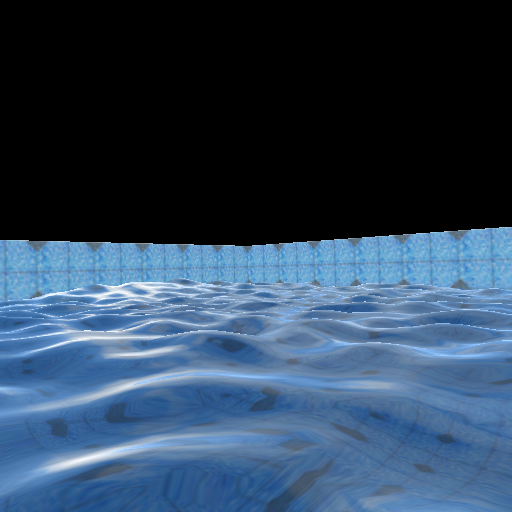
\includegraphics[scale=0.175]{figures/Towards_Real-Time_Visual_Simulation_of_Water_Surfaces_-_Schneider_2001-032.png}
	\label{fig:westermann}
 }
 \hfill
 \subtop[]%[\citeauthor{Isidoro:2002}]
 {
  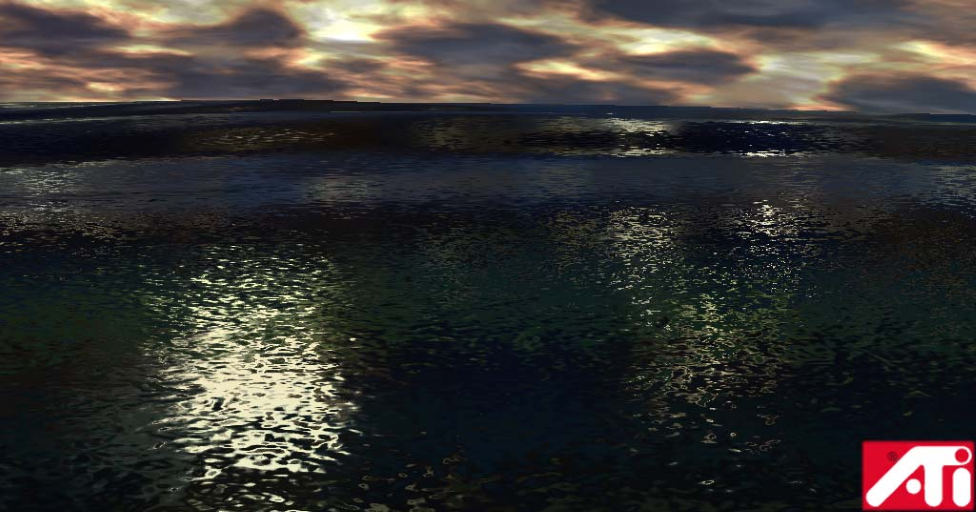
\includegraphics[scale=0.175]{figures/ShaderX_Rendering_Ocean_Water_-_Isidoro_2002-003.png}
	\label{fig:isidoro}
 }
 \hfill
 \subtop[]%[\citeauthor{Finch:2004}]
 {
  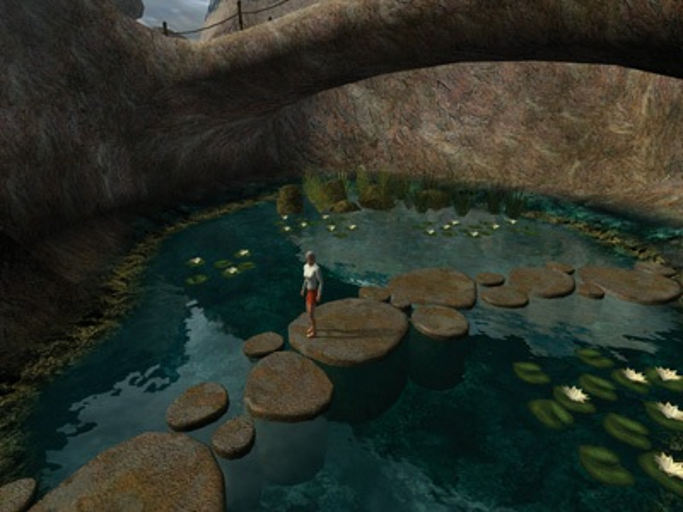
\includegraphics[scale=0.175]{figures/Effective_Water_Simulation_from_Physical_Models_-_Finch_2004-003.png}
	\label{fig:finch}
 }
 \caption{
  Examples of early attempts to generate plausible water surfaces on graphics hardware.
  \subcaptionref{fig:westermann} Source:~\citet{Schneider:2001}
  \subcaptionref{fig:isidoro} Source:~\citet{Isidoro:2002}
  \subcaptionref{fig:finch} Source:~\citet{Finch:2004}
}
\label{fig:earlygpu}
\end{figure}
%
Early attempts to generate plausible water surfaces on graphics hardware include
\citet{Schneider:2001, Isidoro:2002} and \citet{Finch:2004}. Figure~\ref{fig:earlygpu}
depicts some of their results.
To obtain interactive framerates, \citeauthor{Schneider:2001} compute the
displacements caused by wave motion using two octaves of Perlin noise in a
vertex shader on the GPU (Figure~\ref{fig:westermann}).
\citeauthor{Isidoro:2002} perturb an existing mesh by means of a sum of four
low-frequency sinusoids computed in a vertex shader on the GPU
(Figure~\ref{fig:isidoro}). Additional high-frequency detail is obtained by
scrolling static normalmaps across the displaced surface.
%In a similar fashion,
%\cite{Chen:2007} employ a sum of four sinusoids to displace an existing mesh,
%and a dynamically generated normalmap to obtain more detailed surface normals.
\citeauthor{Finch:2004} uses a sum of four Gerstner waves to displace an existing
mesh, where \wavelengths that are too short to be represented by the mesh are
filtered out automatically (Figure~\ref{fig:finch}). Moreover,
\citeauthor{Finch:2004} evaluates an additional sum, with more waves involved,
to generate better detailed surface normals.

%\cite{Salgado:2007} present a simplified implementation of \cite{Fournier:1986}
%using vertex shaders.

\subsection{Adaptive Schemes}
Viewing situations involving an ocean surface are varied: from close-ups where
one may notice ripples on the surface, to views where the water surface may
span until the horizon. Hence, to improve performance and visual fidelity,
it is beneficial for rendering algorithms to focus on regions near the camera
position, minimizing the number of samples according to the distance from the
viewpoint.
%Given a viewing situation where one observes the ocean reaching the horizon, a
%meshing scheme with uniformly spaced vertices in world space may do us a
%disservice. The visible surface area is large and a high resolution is
%needed in regions close to the camera, thus a very large mesh is required.
%
%Minimize the sampling of the geometry according to distance from the viewpoint.
%Mesh adapts to viewing situation
%Simulation adapts to viewing situation
\begin{figure}
 \centering
 \subtop[]%[\citeauthor{Schneider:2001}]
 {
  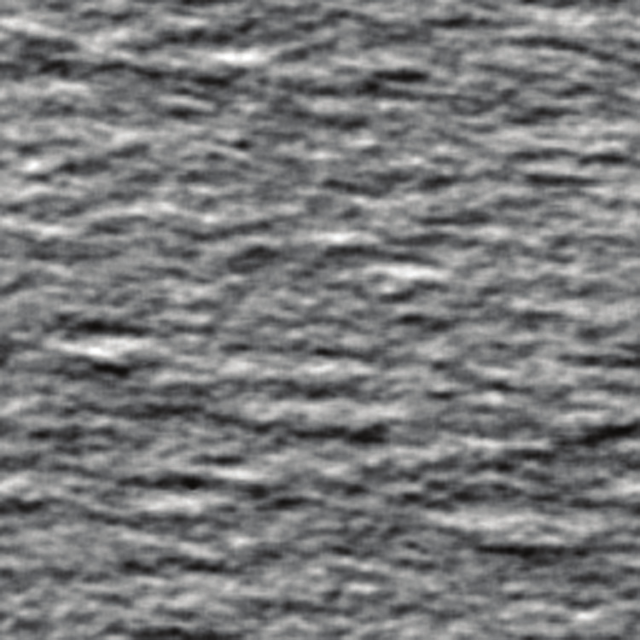
\includegraphics[scale=0.175]{figures/Using_Vertex_Texture_Displacement_for_Realistic_Water_Rendering_-_Kryachko_2005-009.png}
	\label{fig:kryachko:waves}
 }
 \hfill
 \subtop[]%[\citeauthor{Schneider:2001}]
 {
  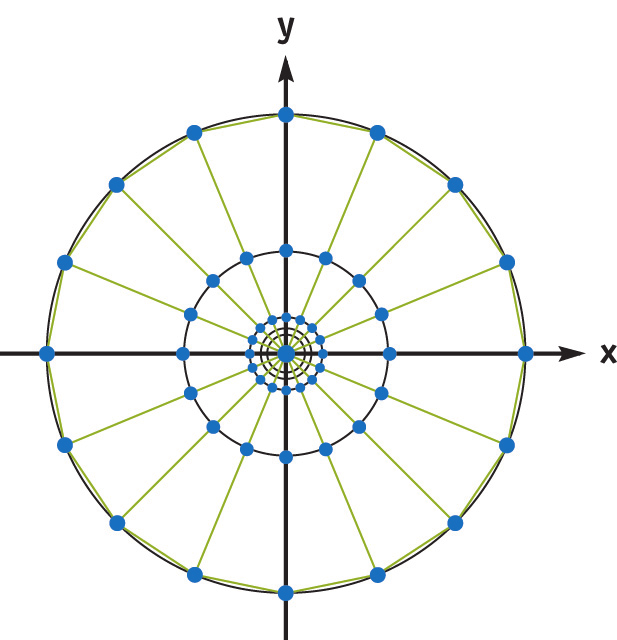
\includegraphics[scale=0.175]{figures/Using_Vertex_Texture_Displacement_for_Realistic_Water_Rendering_-_Kryachko_2005-012.png}
	\label{fig:kryachko:meshing}
 }
 \hfill
 \subtop[]%[\citeauthor{Isidoro:2002}]
 {
  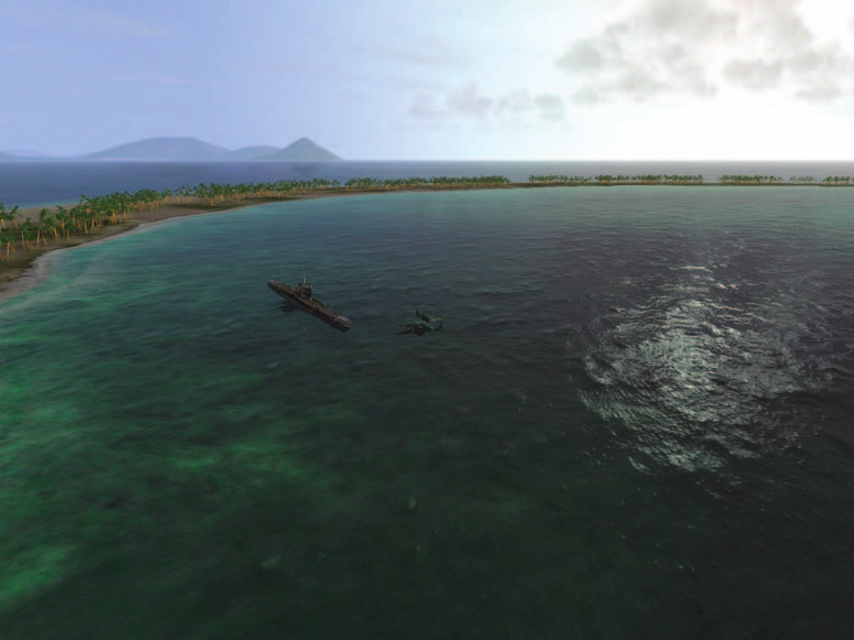
\includegraphics[scale=0.175]{figures/Using_Vertex_Texture_Displacement_for_Realistic_Water_Rendering_-_Kryachko_2005-026.png}
	\label{fig:kryachko:results}
 }
 \caption{
  \subcaptionref{fig:kryachko:waves} A height map used for water displacement.
  \subcaptionref{fig:kryachko:meshing} Radial grid centered at the camera position.
  \subcaptionref{fig:kryachko:results} View with the ocean spanning to the horizon.
  Source:~\cite{Kryachko:2005}
}
\label{fig:kryachko}
\end{figure}
%

\citet{Kryachko:2005} describes the algorithm used in an actual flight simulator.
The ocean is modeled as a combination of handcrafted heightmaps tiled in space
and time (Figure~\ref{fig:kryachko:waves}). Four heightmaps are summed for lighting computations, where two of them
with the largest scale are used to displace the ocean surface mesh. The latter is
organized as a radial grid centered at the camera position, tesselated such that
it provides more detail close to the viewer, see Figure~\ref{fig:kryachko:meshing}.
Radial grid positions are calculated in the vertex shader, as are displacements,
allowing the algorithm to adapt the mesh vertices as well as displacement computations
to the camera position automatically on the GPU for each frame. Still, one may
notice that most of the radial mesh is always outside the view frustum,
causing unnecessary overhead.
%
%
\begin{figure}
 \centering
 \subtop[]
 {
  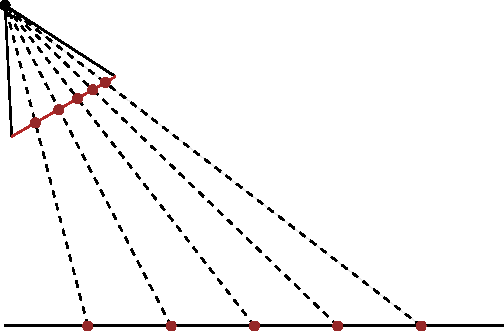
\includegraphics[scale=0.425]{figures/ProjectedGrid_UniformWS.pdf}
  \label{fig:hinsinger:projectedgrid:ws}
 }
 \hfill
 \subtop[]
 {
  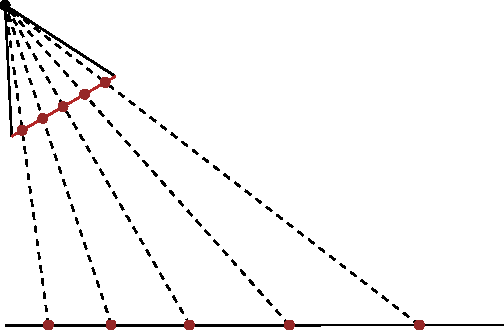
\includegraphics[scale=0.425]{figures/ProjectedGrid_UniformSS.pdf}
  \label{fig:hinsinger:projectedgrid:ss}
 }
 \hfill
 \subtop[]
 {
  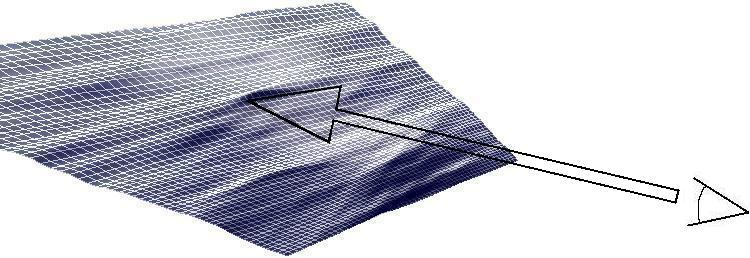
\includegraphics[scale=0.25]{figures/Interactive_Animation_of_Ocean_Waves_-_Hinsinger_2002-003.png}
  \label{fig:hinsinger:projectedgrid:mesh}
 }
 \caption{
  \subcaptionref{fig:hinsinger:projectedgrid:ws} Uniformly spaced vertices in world space, their projection onto the screen is not uniformly spaced though.
  \subcaptionref{fig:hinsinger:projectedgrid:ss} Uniformly spaced vertices in screen space projected onto world space base plane.
  \subcaptionref{fig:hinsinger:projectedgrid:mesh} The result mesh obtained by projection of the vertices onto the base plane followed by displacement.
  One can see that the surface patches grow with distance from the viewer.
  Source:~\cite{Hinsinger:2002}
}
\label{fig:hinsinger:mesh}
\end{figure}
%
%

\citet{Hinsinger:2002} present a more holistic approach, with their contribution
being twofold. One, an adaptive meshing scheme, and two, an adaptive simulation
scheme. The basic idea for the adaptive surface mesh is to make sure that every
surface element at rest covers the same area on screen. Thus, the screen is
subdivided into quads which are projected onto the plane which represents the
ocean surface at rest, see Figure~\ref{fig:hinsinger:mesh}. The result is
a mesh which automatically adapts to the current camera position and gives more
detail close to the viewer.
\citeauthor{Hinsinger:2002} synthesize waves as a sum of Gerstner waves, where
the vertices represent the sampling points. Derivatives are computed analytically
for each vertex, resulting in better normal vectors than a finite differences
approach would produce. To reduce aliasing as well as to save computation time,
wavetrains smaller than a grid quad are removed from the sum of waves for that quad.
% Visual artifacts caused by sampling locations changing with camera movement are
% hidden by the waves animation.
% First, quads in screenspace, projected onto undisturbed surface plane
% change mesh in screenspace to focus on details in certain regions
% water animation hides artifacts caused by moving vertices
% sum of gerstner waves, hand picked, not automatically from spectrum
% analytical derivatives for normals
% prune wavetrains smaller than the grid quads, fade them out
% evaluate surface at any deseired location
% no cyclicity, if ratios between wavelengths irrational
\citet{Cui:2004} uses the adaptive mesh by \citeauthor{Hinsinger:2002} for a marine
simulator with three adjacent viewports, the wave model although is a simple sum
of sinusoids with a small number of waves picked from a wave spectrum.
\citet{thesis:johanson} on the other hand improves upon the adaptive mesh of
\citeauthor{Hinsinger:2002}. First, the projection of the mesh onto the base plane
is moved from the CPU to a vertex shader on the GPU. Second, \citeauthor{thesis:johanson} makes
sure that the projection of the vertices works correctly in all possible viewing
situations.
%
%
\begin{figure}[p]
 \centering
 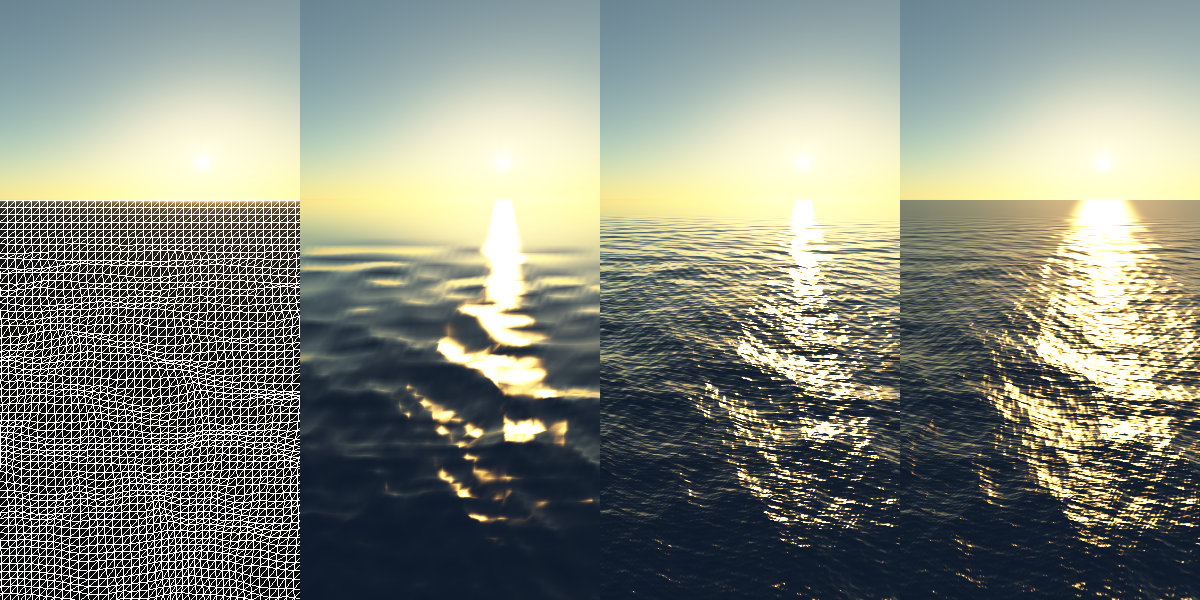
\includegraphics[scale=0.3]{figures/Seamless_Ocean_Lighting_-_Bruneton_2010-001.png}
 \caption{From left to right: The displaced surface mesh in screen space, lighting
 with geometry only, lighting with geometry and per pixel normals, lighting with 
 geometry and per pixel normals and BRDF.
 Source:~\cite{article:oceanlighting}}
\label{fig:bruneton:transitions}
\end{figure}
%
%
\begin{figure}[p]
 \centering
 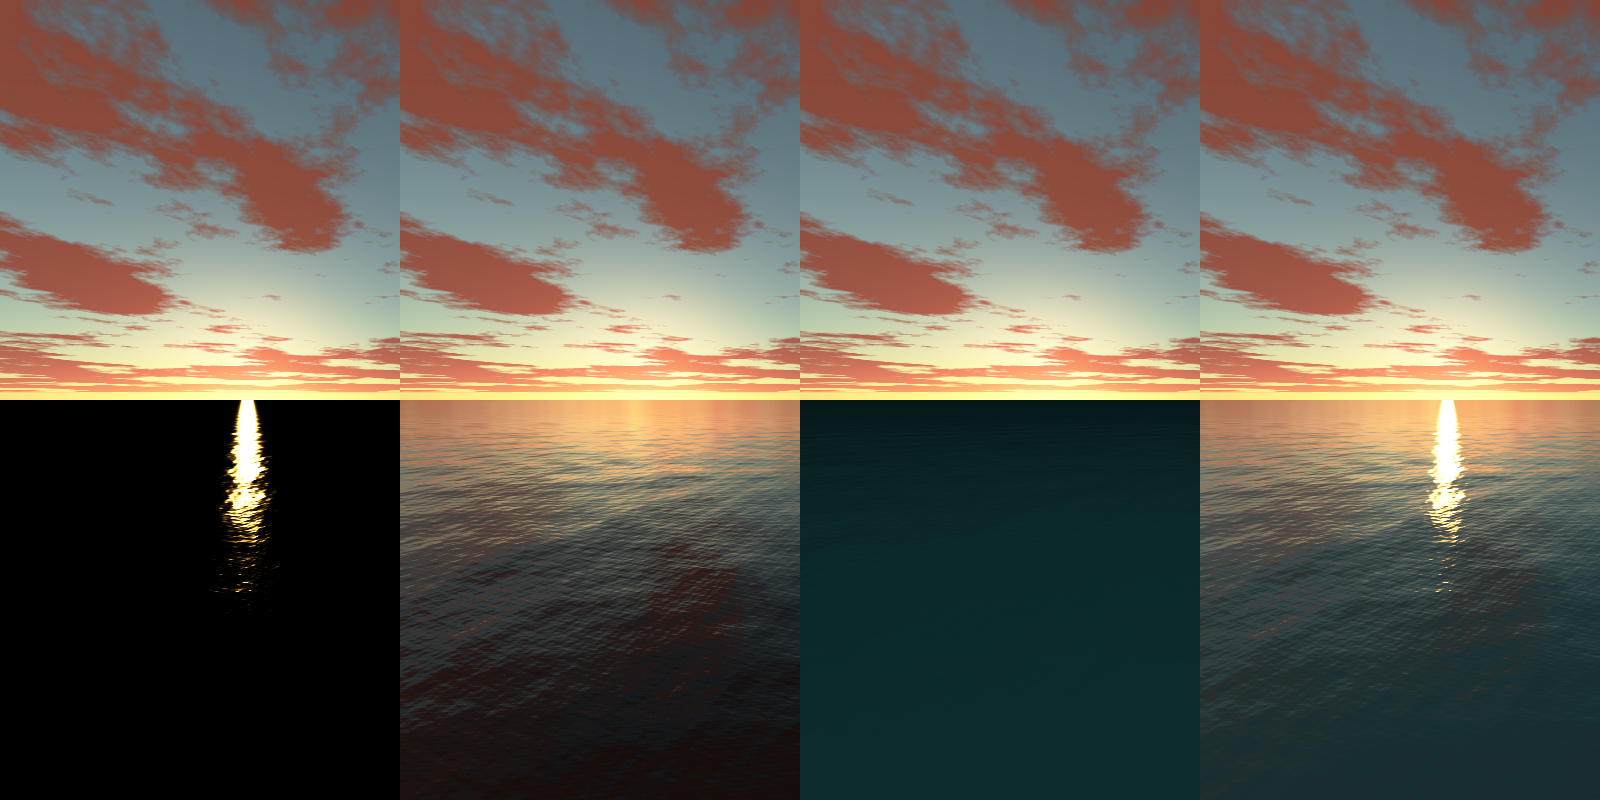
\includegraphics[scale=0.25]{figures/Seamless_Ocean_Lighting_-_Bruneton_2010-002.png}
 \caption{From left to right: The reflected sun light, the reflected sky light,
 the light refracted from the water, and the final result.
 Source:~\cite{article:oceanlighting}}
\label{fig:bruneton:lightingterms}
\end{figure}
%
%

\citet{article:oceanlighting} augment the work of \citeauthor{Hinsinger:2002} in
various areas, the most prominent improvement being an adaptive lighting scheme.
The latter is based on a hierarchical representation which combines geometry,
normals and a BRDF~\citep{Ross:2005}, where the BRDF is specifically tailored to
the statistical properties of ocean surfaces. Based on distance from the viewer,
the algorithm transitions seamlessy from lighting computed with geometry and per
pixel normals to lighting computed based solely on the statistical distribution
of ocean surface slopes as modeled by the BRDF, see Figure~\ref{fig:bruneton:transitions}.
To save computation time for vertex positions, wavetrains are filtered according
to the size of their associated projected grid cell in world space.
For the gradient computation in the pixel shader there is an additional step,
where wavetrains are filtered according to the projected size of the current pixel
in world space. In addition, \citeauthor{article:oceanlighting} show the
integration of the BRDF by \citeauthor{Ross:2005} into the computation of
all necessary lighting terms, namely the reflected light from the sun and from
the skydome, and the refracted light from the water, as seen in
Figure~\ref{fig:bruneton:lightingterms}.
 
% Realistic animation and rendering of the ocean is an important aspect for simulators, movies and video games.
% By nature, the ocean is a difficult problem for Computer Graphics: it is a dynamic system, it combines wave trains
% at all scales, ranging from kilometric to millimetric. Worse, the ocean is usually viewed at several distances, from
% very close to the viewpoint to the horizon, increasing the multi-scale issue, and resulting in aliasing problems. The
% illumination comes from natural light sources (the Sun and the sky dome), is also dynamic, and often underlines
% the aliasing issues. In this paper, we present a new algorithm for modelling, animation, illumination and rendering
% of the ocean, in real-time, at all scales and for all viewing distances. Our algorithm is based on a hierarchical
% representation, combining geometry, normals and BRDF. For each viewing distance, we compute a simplified
% version of the geometry, and encode the missing details into the normal and the BRDF, depending on the level of
% detail required. We then use this hierarchical representation for illumination and rendering. Our algorithm runs
% in real-time, and produces highly realistic pictures and animations.

%Parametric approaches in the spatial domain profit from the fact
%that for each frame only visible parts and frequencies of the ocean surface
%are to be evaluated.
% \citet{Mitchell:2005} and \citet{Thon:2000}
% argue that from an algorithmic point of view one should choose a spectral
% approach and leverage the highly efficient Fast Fourier Transform algorithm
% to compute the sum of waves.
\citet{Mitchell:2005} describes a
partial GPU implementation of the ocean wave generation method presented in
\citet{course:simulatingocean}. To improve rendering performance,
\citeauthor{Mitchell:2005} synthesizes two water surface height maps,
where one contains low frequency waveforms and the other contains
low frequency and high frequency waveforms. The low frequency map
is of low resolution and is used to displace the water surface mesh.
The high resolution map is used to generate a normal map for shading.
The result is an ocean surface which appears highly detailed
while the underlying mesh is coarse.

%
%
\begin{figure}
 \centering
 \renewcommand{\thesubfigure}{}% no subfigure number
 \tightsubcaptions % we want tight subcaptions
 \setlength{\subfloatlabelskip}{0pt}% no space between number and caption
 \subtop[]
 {
  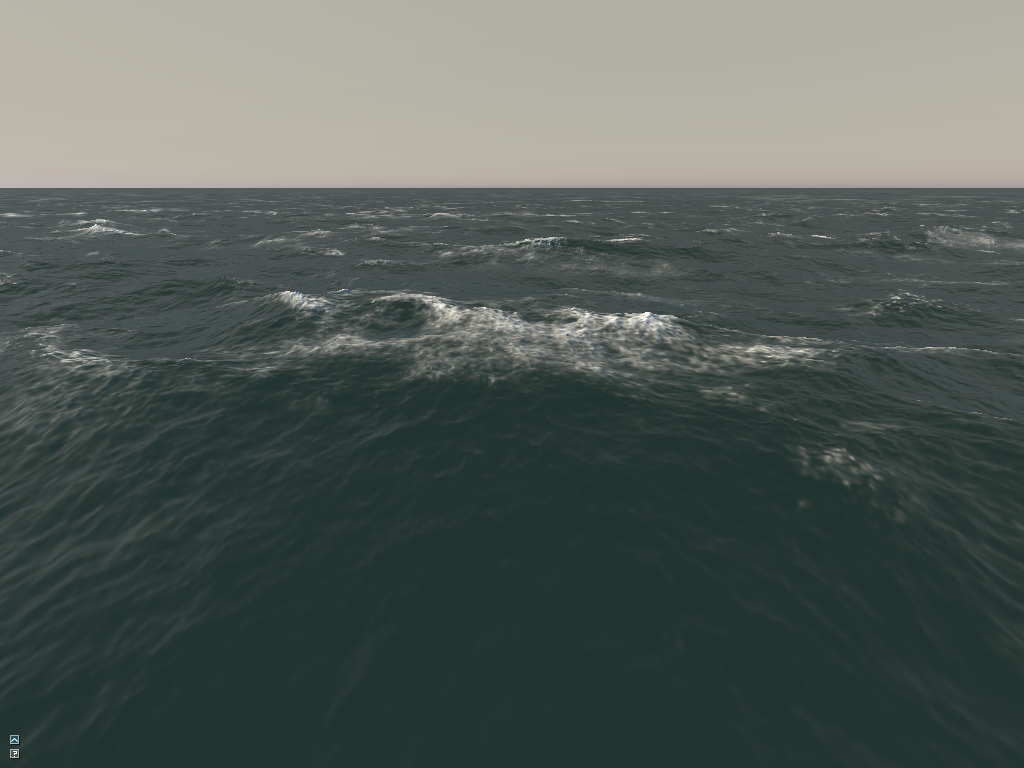
\includegraphics[scale=0.125]{figures/Real-time_Animation_and_Rendering_of_Ocean_Whitecaps-000.png}
  %\label{fig:hinsinger:projectedgrid:ws}
 }
 \hfill
 \subtop[]
 {
  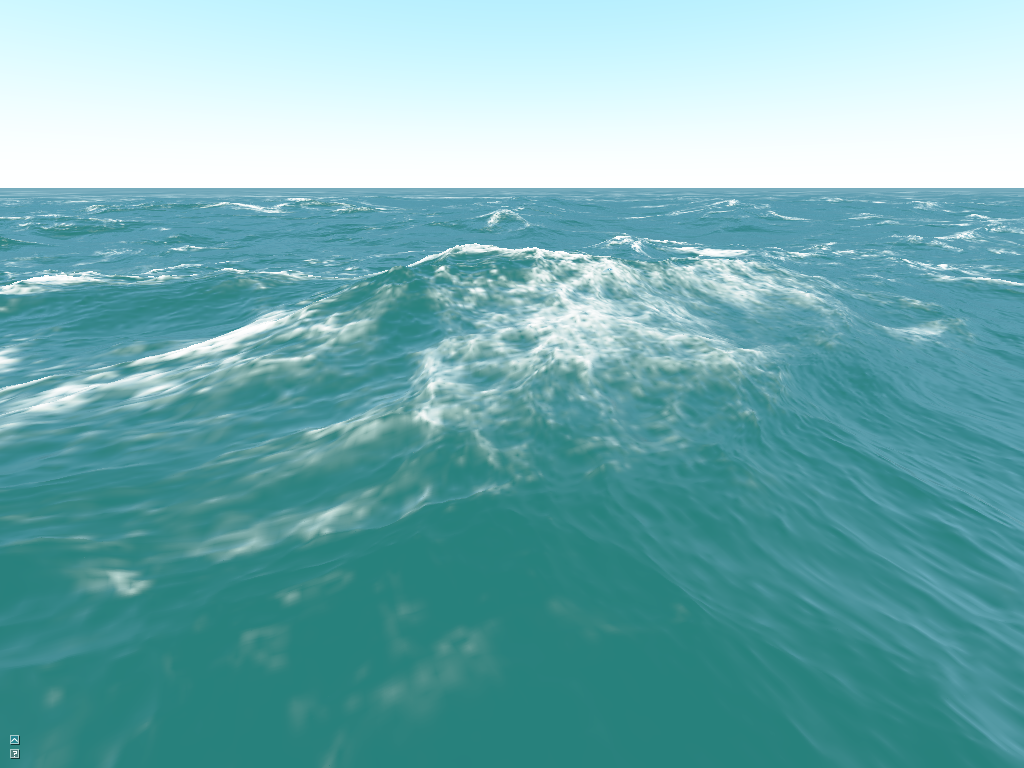
\includegraphics[scale=0.125]{figures/Real-time_Animation_and_Rendering_of_Ocean_Whitecaps-002.png}
  %\label{fig:hinsinger:projectedgrid:ss}
 }
 \hfill
 \subtop[]
 {
  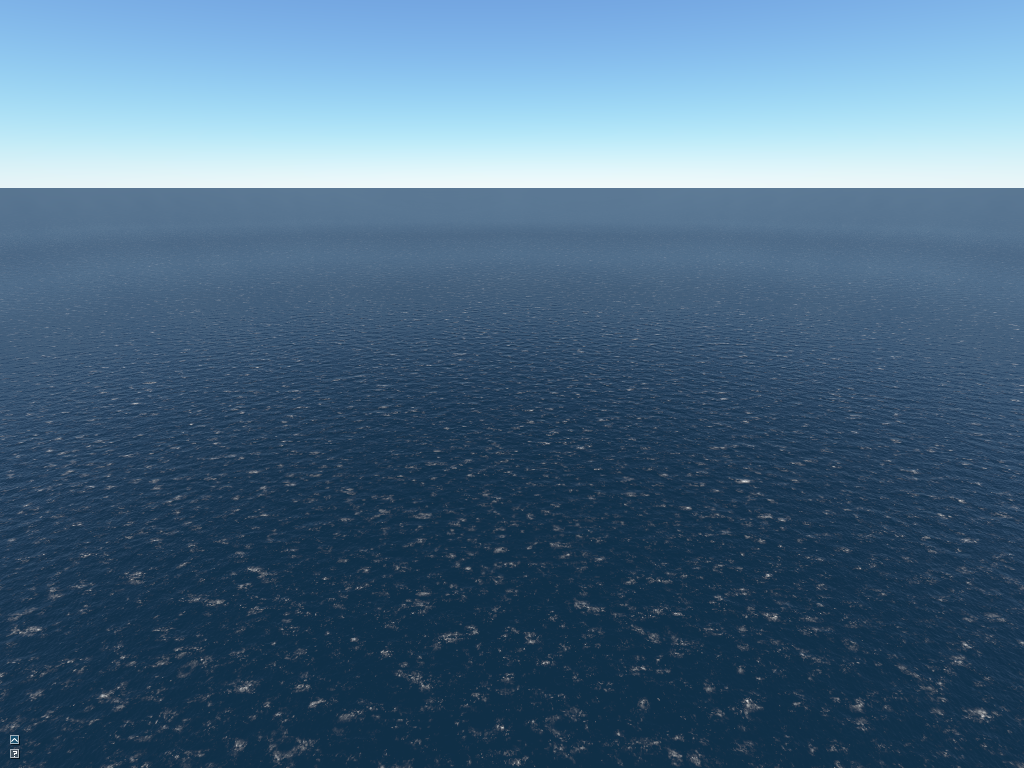
\includegraphics[scale=0.125]{figures/Real-time_Animation_and_Rendering_of_Ocean_Whitecaps-004.png}
  %\label{fig:hinsinger:projectedgrid:mesh}
 }
\caption{A set of example ocean scenes with whitecaps. Source:~\cite{article:whitecaps}
}
\label{fig:dupuy:whitecaps}
\end{figure}
%
%
\citet{misc:oceanlightingfft} combines the adaptive lighting scheme
from \citet{article:oceanlighting} with an ocean surface synthesized
from the wave spectrum presented in~\citet{article:Elfouhaily1997}.
Wave heights, gradients, as well as the horizontal displacements
required for the choppy wave algorithm by \citet{course:simulatingocean}
are computed entirely on the GPU. In an additional step,
\citet{article:whitecaps} add whitecaps to the ocean lighting model,
see Figure~\ref{fig:dupuy:whitecaps}.

As ocean surfaces generated from wave spectra allow for seamless tiling,
one may need to make sure to reduce tiling artifacts i.e. the viewer
shall not notice that the ocean surface repeats itself in all directions.
The approach taken by~\citet{Rydahl:2009} and \citet{NVIDIA:Ocean} is to
generate additional noise on the ocean surface.
\citet{misc:oceanlightingfft} and \citet{article:whitecaps}
on the other hand compute not just one ocean surface tile, but up to four,
where all tiles are of different size and each one samples a different
part of the wave spectrum. Even though such an approach is unable to
entirely remove periodicity, the period is increased to the least common
multiple of the different tile sizes.
